\chapter{Corelations: a tool for black boxing} \label{ch.corelations}

As we have seen, cospans are a useful tool for describing finite colimits, and
so for describing the interconnection of systems. In the previous chapter
we defined decorated cospans to take advantage of this fact and provide
a tool for composing structures that had no inherent composition law, like
graphs and subspaces. In many situations, however, the colimit contains more
information than we care about.  Rather than concerning ourselves with all the
internal structure of a system, we only find a certain aspect of it
relevant---roughly, the part that affects what happens at the boundary. This is
better modelled by corelations. In this chapter we develop the theory of
corelations.

As usual, we begin by giving an intuitive overview of the aims of this chapter
in \textsection\ref{sec.blackboxing}. We then give the formal details of
corelation categories (\textsection\ref{sec.corels}) and their functors
(\textsection\ref{sec.corelfunctors}), before concluding in
\textsection\ref{sec.corelexs} with two important
examples: equivalence relations as epi-mono corelations in $(\Set,+)$, and
linear relations as epi-mono corelations in $(\Vect,\oplus)$. This sets us up
for a decorated version of this theory in Chapter \ref{ch.deccorels}.

\section{The idea of black boxing} \label{sec.blackboxing}

Thus far we have argued that network languages should be modelled using
hypergraph categories, and shown that cospans provide a good language for
talking about interconnection. We then developed the theory of decorated
cospans, which allows us to take diagrams, mark `inputs' and `outputs' using
cospans, and then compose these diagrams using pushouts. This turns a notion of
closed system into a notion of open one.

A serious limitation of using cospans alone, however, is that cospans
indiscrimately accumulate information. For example, suppose we consider the
morphisms of $\mathrm{GraphCospan}$ as open electrical circuits as in
\textsection\ref{ssec.exelectricalcircuits}. Pursuing this, let us depict a
graph decorated cospan from $(X \xrightarrow{i} N \xleftarrow{o} Y, \enspace
(N,E,s,t,r))$ by 
\[
\resizebox{.35\textwidth}{!}{
    \tikzset{every path/.style={line width=1.1pt}}
  \begin{tikzpicture}[circuit ee IEC, set resistor graphic=var resistor IEC graphic]
	\begin{pgfonlayer}{nodelayer}
		\node [style=dot] (0) at (-2.5, 0.75) {};
		\coordinate (1) at (-2, -2) {};
		\coordinate (2) at (1.5, 2) {};
		\coordinate (A) at (-2, 0.75) {};
		\node [style=dot] (4) at (2, 1.25) {};
		\coordinate (B) at (1.5, 0.75) {};
		\node [style=dot] (6) at (2, 0.25) {};
		\coordinate (ub) at (0.75, 1) {};
		\coordinate (la) at (-1.25, 0.5) {};
		\coordinate (C) at (-0.25, -1.375) {};
		\coordinate (lb) at (0.75, 0.5) {};
		\coordinate (ua) at (-1.25, 1) {};
	\end{pgfonlayer}
	\begin{pgfonlayer}{edgelayer}
		\draw (0.center) to (A);
		\draw (6) to (B);
		\draw (4) to (B);
    \path (A) edge (ua);
    \path (A) edge (la);
    \path (B) edge (ub);
    \path (B) edge (lb);
    \path (ua) edge  [resistor] (ub);
    \path (la) edge  [resistor] (lb);
    \path (A) edge  [resistor]  (C);
    \path (C) edge  [resistor]  (B);
	\end{pgfonlayer}
	\begin{pgfonlayer}{background}
	  \filldraw [fill=black!5!white, draw=black!40!white] (1) rectangle (2);
	\end{pgfonlayer}
\end{tikzpicture}
}
\]
where the bullets $\bullet$ on the left represent the elements of the set $X$,
those on the right represent the elements of $Y$, and we draw a line from $x \in
X$ or $y \in Y$ to a node $n$ in the graph when $i(x) = n$ or $o(y)=n$.  We omit
the labels (resistances) on the edges as these are not essential to the main
point here.  

We also depict an example of composition of these open circuits using decorated
cospans:
\[
\begin{aligned}
\resizebox{.45\textwidth}{!}{
    \tikzset{every path/.style={line width=1.1pt}}
  \begin{tikzpicture}[circuit ee IEC, set resistor graphic=var resistor IEC graphic]
	\begin{pgfonlayer}{nodelayer}
		\node [style=dotbig] (0) at (-2.25, 4) {};
		\coordinate (1) at (-1.75, 1.25) {};
		\coordinate (2) at (1.75, 5.25) {};
		\coordinate (3) at (-1.75, 4) {};
		\node [style=dotbig] (4) at (2.25, 4.5) {};
		\coordinate (5) at (1.75, 4) {};
		\node [style=dotbig] (6) at (2.25, 3.5) {};
		\coordinate (7) at (1, 4.25) {};
		\coordinate (8) at (-1, 3.75) {};
		\coordinate (9) at (0, 1.75) {};
		\coordinate (10) at (1, 3.75) {};
		\coordinate (11) at (-1, 4.25) {};
		\node [style=dotbig] (12) at (7.25, 4) {};
		\coordinate (13) at (-3, -1.5) {};
		\coordinate (14) at (6, 2) {};
		\coordinate (15) at (3.5, 2) {};
		\coordinate (16) at (4.75, -0) {};
		\coordinate (17) at (3, 3.5) {};
		\coordinate (18) at (3, 4.5) {};
		\node [style=dotbig] (19) at (2.5, -1.5) {};
		\coordinate (20) at (6.75, 4) {};
		\node [style=dotbig] (21) at (7.25, -1.5) {};
		\node [style=dotbig] (22) at (-6.5, -1) {};
		\node [style=dotbig] (23) at (7.25, 1.5) {};
		\node [style=dotbig] (24) at (-6.5, 4.5) {};
		\node [style=dotbig] (25) at (-6.5, 3) {};
		\coordinate (26) at (-6, -2) {};
		\coordinate (27) at (-3, 5.25) {};
		\coordinate (28) at (1.75, 1) {};
		\coordinate (29) at (-1.75, -2) {};
		\coordinate (30) at (3, -2) {};
		\coordinate (31) at (-6, 4.5) {};
		\coordinate (32) at (-6, 3) {};
		\coordinate (33) at (-3, 4) {};
		\coordinate (34) at (6.75, 2.5) {};
		\coordinate (35) at (3, 2.75) {};
		\coordinate (36) at (6.75, 5.25) {};
		\node [style=dotbig] (37) at (7.25, 0.5) {};
		\node [style=dotbig] (38) at (-2.25, -1.5) {};
		\node [style=dotbig] (39) at (-2.5, 4) {};
		\node [style=dotbig] (40) at (2.5, 4.5) {};
		\node [style=dotbig] (41) at (2.5, 3.5) {};
		\node [style=dotbig] (42) at (-2.25, 0.5) {};
		\node [style=dotbig] (43) at (-2.5, -1.5) {};
		\node [style=dotbig] (44) at (-2.5, 0.5) {};
		\node [style=dotbig] (45) at (2.25, -1.5) {};
		\node [style=dotbig] (46) at (2.25, -0) {};
		\node [style=dotbig] (47) at (2.5, -0) {};
		\node [style=dotbig] (48) at (-2.5, -0.5) {};
		\node [style=dotbig] (49) at (-2.25, -0.5) {};
		\coordinate (50) at (-6, -1) {};
		\coordinate (51) at (-5, -0) {};
		\coordinate (52) at (-3, 0.5) {};
		\coordinate (53) at (-3, -0.5) {};
		\coordinate (54) at (-1.75, 0.5) {};
		\coordinate (55) at (-1.75, -0.5) {};
		\coordinate (56) at (0, -0) {};
		\coordinate (57) at (1.75, -0) {};
		\coordinate (58) at (3, -0) {};
		\coordinate (59) at (-5.75, 1.25) {};
		\coordinate (60) at (4.75, 1) {};
		\coordinate (61) at (6.75, 1.5) {};
		\coordinate (62) at (6.75, 0.5) {};
		\coordinate (63) at (-1.75, -1.5) {};
		\coordinate (64) at (1.75, -1.5) {};
		\coordinate (65) at (3, -1.5) {};
		\coordinate (66) at (6.75, -1.5) {};
		\coordinate (67) at (-5.5, 1.75) {};
		\coordinate (68) at (-5.25, 1) {};
		\coordinate (69) at (-3.75, 2.5) {};
		\coordinate (70) at (-3.5, 1.75) {};
		\coordinate (71) at (-3.25, 2.25) {};
	\end{pgfonlayer}
	\begin{pgfonlayer}{edgelayer}
		\path (50) edge [resistor] (13);
		\draw (24) to (31);
		\draw (61) to (23);
		\draw (62) to (37);
		\draw (25) to (32);
		\draw (22) to (50);
		\draw (33) to (39);
		\draw (0) to (3);
		\draw (52) to (44);
		\draw (42) to (54);
		\draw (53) to (48);
		\draw (49) to (55);
		\path (31) edge [resistor] (33);
		\path (32) edge [resistor] (33);
		\draw (3) to (11);
		\draw (3) to (8);
		\path (11) edge [resistor] (7);
		\path (8) edge [resistor] (10);
		\draw (7) to (5);
		\draw (10) to (5);
		\draw (5) to (4);
		\draw (5) to (6);
		\draw (41) to (17);
		\draw (40) to (18);
		\path (18) edge [resistor] (20);
		\path (17) edge [resistor] (20);
		\draw (20) to (12);
		\path (15) edge [resistor] (14);
		\path (54) edge [resistor] (56);
		\path (55) edge [resistor] (56);
		\path (56) edge [resistor] (57);
		\path (51) edge [resistor] (52);
		\path (51) edge [resistor] (53);
		\draw (57) to (46);
		\draw (47) to (58);
		\path (58) edge [resistor] (16);
		\path (3) edge [resistor] (9);
		\path (9) edge [resistor] (5);
		\draw (13) to (43);
		\path (60) edge [resistor] (61);
		\path (60) edge [resistor] (62);
		\draw (38) to (63);
		\path (63) edge [resistor] (64);
		\draw (64) to (45);
		\draw (19) to (65);
		\path (65) edge [resistor] (66);
		\draw (66) to (21);
		\path (67) edge [resistor] (69);
		\path (68) edge [resistor] (70);
		\draw (59) to (67);
		\draw (59) to (68);
		\draw (69) to (71);
		\draw (71) to (70);
	\end{pgfonlayer}
	\begin{pgfonlayer}{background}
	  \filldraw [fill=black!5!white, draw=black!40!white] (1) rectangle (2);
	  \filldraw [fill=black!5!white, draw=black!40!white] (26) rectangle (27);
	  \filldraw [fill=black!5!white, draw=black!40!white] (29) rectangle (28);
	  \filldraw [fill=black!5!white, draw=black!40!white] (35) rectangle (36);
	  \filldraw [fill=black!5!white, draw=black!40!white] (30) rectangle (34);
	\end{pgfonlayer}
\end{tikzpicture}
}
\end{aligned}
\quad
\mapsto
\enspace
\begin{aligned}
\resizebox{.4\textwidth}{!}{
    \tikzset{every path/.style={line width=1.1pt}}
  \begin{tikzpicture}[circuit ee IEC, set resistor graphic=var resistor IEC graphic]
	\begin{pgfonlayer}{nodelayer}
		\coordinate (0) at (-1.75, 4) {};
		\coordinate (1) at (1.75, 4) {};
		\coordinate (2) at (1, 4.25) {};
		\coordinate (3) at (-1, 3.75) {};
		\coordinate (4) at (0, 1.75) {};
		\coordinate (5) at (1, 3.75) {};
		\coordinate (6) at (-1, 4.25) {};
		\node [style=dotbig] (7) at (6.25, 4) {};
		\coordinate (8) at (5, 2) {};
		\coordinate (9) at (2.5, 2) {};
		\coordinate (10) at (3.75, -0) {};
		\coordinate (11) at (2.5, 3.75) {};
		\coordinate (12) at (2.5, 4.25) {};
		\coordinate (13) at (5.75, 4) {};
		\node [style=dotbig] (14) at (6.25, -1.5) {};
		\node [style=dotbig] (15) at (-5.5, -1) {};
		\node [style=dotbig] (16) at (6.25, 1.5) {};
		\node [style=dotbig] (17) at (-5.5, 4.5) {};
		\node [style=dotbig] (18) at (-5.5, 3) {};
		\coordinate (19) at (-5, -2) {};
		\coordinate (20) at (-5, 4.5) {};
		\coordinate (21) at (-5, 3) {};
		\coordinate (22) at (5.75, 5.25) {};
		\node [style=dotbig] (23) at (6.25, 0.5) {};
		\coordinate (24) at (-5, -1) {};
		\coordinate (25) at (-4, -0) {};
		\coordinate (26) at (-1.75, 0.5) {};
		\coordinate (27) at (-1.75, -0.5) {};
		\coordinate (28) at (0, -0) {};
		\coordinate (29) at (1.75, -0) {};
		\coordinate (30) at (-4.75, 1.25) {};
		\coordinate (31) at (3.75, 1) {};
		\coordinate (32) at (5.75, 1.5) {};
		\coordinate (33) at (5.75, 0.5) {};
		\coordinate (34) at (-1.75, -1.5) {};
		\coordinate (35) at (1.75, -1.5) {};
		\coordinate (36) at (5.75, -1.5) {};
		\coordinate (37) at (-4.25, 1.75) {};
		\coordinate (38) at (-4.25, 1) {};
		\coordinate (39) at (-2.75, 2.5) {};
		\coordinate (40) at (-2.5, 1.75) {};
		\coordinate (41) at (-2.25, 2.25) {};
		\coordinate (42) at (5, 4.25) {};
		\coordinate (43) at (5, 3.75) {};
	\end{pgfonlayer}
	\begin{pgfonlayer}{edgelayer}
		\draw (17) to (20);
		\draw (18) to (21);
		\draw (15) to (24);
		\draw (13) to (7);
		\draw (36) to (14);
		\draw (32) to (16);
		\draw (33) to (23);
		\draw (1) to (12);
		\draw (1) to (11);
		\draw (2) to (1);
		\draw (5) to (1);
		\draw (0) to (6);
		\draw (0) to (3);
		\draw (30) to (37);
		\draw (30) to (38);
		\draw (39) to (41);
		\draw (41) to (40);
		\draw (42) to (13);
		\draw (43) to (13);
		\path (6) edge [resistor] (2);
		\path (3) edge [resistor] (5);
		\path (9) edge [resistor] (8);
		\path (26) edge [resistor] (28);
		\path (27) edge [resistor] (28);
		\path (28) edge [resistor] (29);
		\path (0) edge [resistor] (4);
		\path (4) edge [resistor] (1);
		\path (31) edge [resistor] (32);
		\path (31) edge [resistor] (33);
		\path (34) edge [resistor] (35);
		\path (37) edge [resistor] (39);
		\path (38) edge [resistor] (40);
		\path (20) edge [resistor] (0);
		\path (21) edge [resistor] (0);
		\path (25) edge [resistor] (26);
		\path (25) edge [resistor] (27);
		\path (24) edge [resistor] (34);
		\path (29) edge [resistor] (10);
		\path (35) edge [resistor] (36);
		\path (12) edge [resistor] (42);
		\path (11) edge [resistor] (43);
	\end{pgfonlayer}
	\begin{pgfonlayer}{background}
	  \filldraw [fill=black!5!white, draw=black!40!white] (19) rectangle (22);
	\end{pgfonlayer}
\end{tikzpicture}
}
\end{aligned}
\]
Note in particular that the composite of these open circuits contains a unique
resistor for every resistor in the factors. If we are interested in describing
the syntax of a diagrammatic language, then this is useful: composition builds
given expressions into a larger one. If we are only interested in the semantics,
however, this is often unnecessary and thus often wildly inefficient.

Indeed, suppose our semantics for open circuits is given by the information that
can be gleaned by connecting other open circuits, such as measurement devices,
to the terminals. In these semantics we consider two open circuits equivalent
if, should they be encased, but for their terminals, in a black box
\[
\resizebox{.4\textwidth}{!}{
    \tikzset{every path/.style={line width=1.1pt}}
  \begin{tikzpicture}
    \begin{pgfonlayer}{nodelayer}
		\node [style=dotbig] (14) at (-5.5, 4.5) {};
		\node [style=dotbig] (15) at (-5.5, 3) {};
		\node [style=dotbig] (12) at (-5.5, -1) {};
		\node [style=dotbig] (7) at (6.25, 4) {};
		\node [style=dotbig] (13) at (6.25, 1.5) {};
		\node [style=dotbig] (20) at (6.25, 0.5) {};
		\node [style=dotbig] (11) at (6.25, -1.5) {};
		\coordinate (17) at (-5, 4.5) {};
		\coordinate (18) at (-5, 3) {};
		\coordinate (21) at (-5, -1) {};
		\coordinate (10) at (5.75, 4) {};
		\coordinate (23) at (5.75, 1.5) {};
		\coordinate (24) at (5.75, 0.5) {};
		\coordinate (27) at (5.75, -1.5) {};
		\coordinate (16) at (-5, -2) {};
		\coordinate (19) at (5.75, 5.25) {};
	\end{pgfonlayer}
	\begin{pgfonlayer}{edgelayer}
		\draw (14) to (17);
		\draw (15) to (18);
		\draw (12) to (21);
		\draw (10) to (7);
		\draw (27) to (11);
		\draw (23) to (13);
		\draw (24) to (20);
	\end{pgfonlayer}
	\begin{pgfonlayer}{background}
	  \filldraw [fill=black!80!white, draw=black!40!white] (16) rectangle (19);
	\end{pgfonlayer}
\end{tikzpicture}
}
\]
we would be unable to distinguish them through our electrical investigations. In
this case, at the very least, the previous circuit is equivalent to the circuit
\[
\resizebox{.4\textwidth}{!}{
    \tikzset{every path/.style={line width=1.1pt}}
  \begin{tikzpicture}[circuit ee IEC, set resistor graphic=var resistor IEC graphic]
	\begin{pgfonlayer}{nodelayer}
		\coordinate (0) at (-1.75, 4) {};
		\coordinate (1) at (1.75, 4) {};
		\coordinate (2) at (1, 4.25) {};
		\coordinate (3) at (-1, 3.75) {};
		\coordinate (4) at (0, 1.75) {};
		\coordinate (5) at (1, 3.75) {};
		\coordinate (6) at (-1, 4.25) {};
		\node [style=dotbig] (7) at (6.25, 4) {};
		\coordinate (8) at (2.5, 3.75) {};
		\coordinate (9) at (2.5, 4.25) {};
		\coordinate (10) at (5.75, 4) {};
		\node [style=dotbig] (11) at (6.25, -1.5) {};
		\node [style=dotbig] (12) at (-5.5, -1) {};
		\node [style=dotbig] (13) at (6.25, 1.5) {};
		\node [style=dotbig] (14) at (-5.5, 4.5) {};
		\node [style=dotbig] (15) at (-5.5, 3) {};
		\coordinate (16) at (-5, -2) {};
		\coordinate (17) at (-5, 4.5) {};
		\coordinate (18) at (-5, 3) {};
		\coordinate (19) at (5.75, 5.25) {};
		\node [style=dotbig] (20) at (6.25, 0.5) {};
		\coordinate (21) at (-5, -1) {};
		\coordinate (22) at (3.75, 1) {};
		\coordinate (23) at (5.75, 1.5) {};
		\coordinate (24) at (5.75, 0.5) {};
		\coordinate (25) at (-1.75, -1.5) {};
		\coordinate (26) at (1.75, -1.5) {};
		\coordinate (27) at (5.75, -1.5) {};
		\coordinate (28) at (5, 4.25) {};
		\coordinate (29) at (5, 3.75) {};
	\end{pgfonlayer}
	\begin{pgfonlayer}{edgelayer}
		\draw (14) to (17);
		\draw (15) to (18);
		\draw (12) to (21);
		\draw (10) to (7);
		\draw (27) to (11);
		\draw (23) to (13);
		\draw (24) to (20);
		\draw (1) to (9);
		\draw (1) to (8);
		\draw (2) to (1);
		\draw (5) to (1);
		\draw (0) to (6);
		\draw (0) to (3);
		\draw (28) to (10);
		\draw (29) to (10);
		\path (6) edge [resistor] (2);
		\path (3) edge [resistor] (5);
		\path (0) edge [resistor] (4);
		\path (4) edge [resistor] (1);
		\path (22) edge [resistor] (23);
		\path (22) edge [resistor] (24);
		\path (25) edge [resistor] (26);
		\path (17) edge [resistor] (0);
		\path (18) edge [resistor] (0);
		\path (21) edge [resistor] (25);
		\path (26) edge [resistor] (27);
		\path (9) edge [resistor] (28);
		\path (8) edge [resistor] (29);
	\end{pgfonlayer}
	\begin{pgfonlayer}{background}
	  \filldraw [fill=black!5!white, draw=black!40!white] (16) rectangle (19);
	\end{pgfonlayer}
\end{tikzpicture}
}
\]
where we have removed circuitry not connected to the terminals.  Moreover, this
second circuit is a much more efficient representation, as it does not model
inaccessible, internal structure. If we wish to construct a hypergraph category
modelling the semantics of open circuits, we require circuit representations and
a composition rule that only retain the information relevant to the black boxed
circuit.

Dealing with this problem fully requires further discussion of the semantics of
circuit diagrams, and the introduction of structures more flexible than graphs,
such as linear relations.  We deal with this in depth in Chapter
\ref{ch.circuits}. In this chapter, however, we are able to contribute an
important piece of the puzzle: corelations.

Corelations allow us to pursue a notion of composition that discards extraneous
information as we compose our systems. Consider, for example, the category
$\cospan(\FinSet)$ of cospans in the category of finite sets and functions. A
morphism is then a finite set $N$ together with functions $X \to N$ and $Y \to
N$. We depict these like so:
\begin{center}
  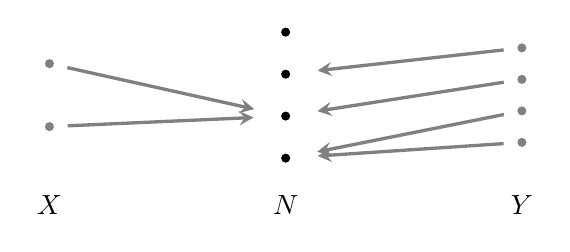
\begin{tikzpicture}[auto,scale=2]
    \node[circle,draw,inner sep=1pt,fill=gray,color=gray] (x1) at (-1.5,.2) {};
    \node[circle,draw,inner sep=1pt,fill=gray,color=gray] (x2) at (-1.5,-.2) {};
    \node at (-1.5,-.7) {$X$};
    \node[circle,draw,inner sep=1pt,fill]         (A) at (0,.4) {};
    \node[circle,draw,inner sep=1pt,fill]         (B) at (0,.133) {};
    \node[circle,draw,inner sep=1pt,fill]         (C) at (0,-.133) {};
    \node[circle,draw,inner sep=1pt,fill]         (D) at (0,-.4) {};
    \node at (0,-.7) {$N$};
    \node[circle,draw,inner sep=1pt,fill=gray,color=gray] (y1) at (1.5,.3) {};
    \node[circle,draw,inner sep=1pt,fill=gray,color=gray] (y2) at (1.5,.1) {};
    \node[circle,draw,inner sep=1pt,fill=gray,color=gray] (y3) at (1.5,-.1) {};
    \node[circle,draw,inner sep=1pt,fill=gray,color=gray] (y4) at (1.5,-.3) {};
    \node at (1.5,-.7) {$Y$};
    \path[color=gray, very thick, shorten >=10pt, shorten <=5pt, ->, >=stealth]
    (x1) edge (C);
    \path[color=gray, very thick, shorten >=10pt, shorten <=5pt, ->, >=stealth]
    (x2) edge (C);
    \path[color=gray, very thick, shorten >=10pt, shorten <=5pt, ->, >=stealth]
    (y1) edge (B);
    \path[color=gray, very thick, shorten >=10pt, shorten <=5pt, ->, >=stealth]
    (y2) edge (C);
    \path[color=gray, very thick, shorten >=10pt, shorten <=5pt, ->, >=stealth]
    (y3) edge (D);
    \path[color=gray, very thick, shorten >=10pt, shorten <=5pt, ->, >=stealth]
    (y4) edge (D);
  \end{tikzpicture}
\end{center}
Here $X$ is a two element set, while $N$ and $Y$ are four element sets.

Suppose we have a pair of cospans $X \to N \leftarrow Y$, $Y \to M \leftarrow
Z$. By definition, their composite has apex the pushout $N+_YM$ which, roughly
speaking, is the union of $N$ and $M$ with two points identified if they are
both images of the same element of $Y$. For example, the following pair of
cospans:
\begin{center}
  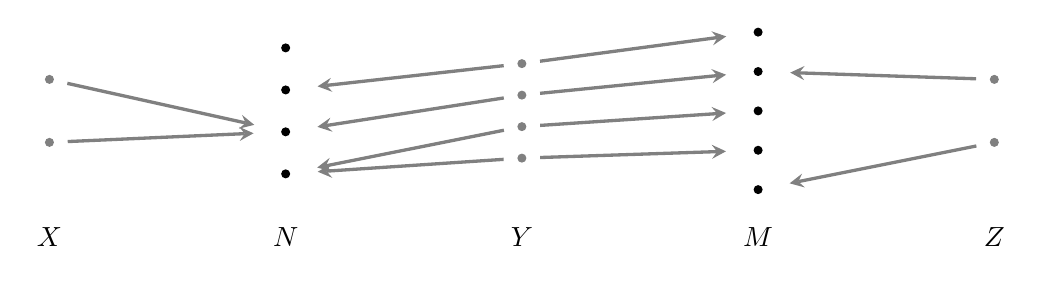
\begin{tikzpicture}[auto,scale=2]
    \node[circle,draw,inner sep=1pt,fill=gray,color=gray] (x1) at (-1.5,.2) {};
    \node[circle,draw,inner sep=1pt,fill=gray,color=gray] (x2) at (-1.5,-.2) {};
    \node at (-1.5,-.8) {$X$};
    \node[circle,draw,inner sep=1pt,fill]         (A) at (0,.4) {};
    \node[circle,draw,inner sep=1pt,fill]         (B) at (0,.133) {};
    \node[circle,draw,inner sep=1pt,fill]         (C) at (0,-.133) {};
    \node[circle,draw,inner sep=1pt,fill]         (D) at (0,-.4) {};
    \node at (0,-.8) {$N$};
    \node[circle,draw,inner sep=1pt,fill=gray,color=gray] (y1) at (1.5,.3) {};
    \node[circle,draw,inner sep=1pt,fill=gray,color=gray] (y2) at (1.5,.1) {};
    \node[circle,draw,inner sep=1pt,fill=gray,color=gray] (y3) at (1.5,-.1) {};
    \node[circle,draw,inner sep=1pt,fill=gray,color=gray] (y4) at (1.5,-.3) {};
    \node at (1.5,-.8) {$Y$};
    \node[circle,draw,inner sep=1pt,fill]         (A') at (3,.5) {};
    \node[circle,draw,inner sep=1pt,fill]         (B') at (3,.25) {};
    \node[circle,draw,inner sep=1pt,fill]         (C') at (3,0) {};
    \node[circle,draw,inner sep=1pt,fill]         (D') at (3,-.25) {};
    \node[circle,draw,inner sep=1pt,fill]         (E') at (3,-.5) {};
    \node at (3,-.8) {$M$};
    \node[circle,draw,inner sep=1pt,fill=gray,color=gray] (z1) at (4.5,.2) {};
    \node[circle,draw,inner sep=1pt,fill=gray,color=gray] (z2) at (4.5,-.2) {};
    \node at (4.5,-.8) {$Z$};
    \path[color=gray, very thick, shorten >=10pt, shorten <=5pt, ->, >=stealth]
    (x1) edge (C);
    \path[color=gray, very thick, shorten >=10pt, shorten <=5pt, ->, >=stealth]
    (x2) edge (C);
    \path[color=gray, very thick, shorten >=10pt, shorten <=5pt, ->, >=stealth]
    (y1) edge (B);
    \path[color=gray, very thick, shorten >=10pt, shorten <=5pt, ->, >=stealth]
    (y2) edge (C);
    \path[color=gray, very thick, shorten >=10pt, shorten <=5pt, ->, >=stealth]
    (y3) edge (D);
    \path[color=gray, very thick, shorten >=10pt, shorten <=5pt, ->, >=stealth]
    (y4) edge (D);
    \path[color=gray, very thick, shorten >=10pt, shorten <=5pt, ->, >=stealth]
    (y1) edge (A');
    \path[color=gray, very thick, shorten >=10pt, shorten <=5pt, ->, >=stealth]
    (y2) edge (B');
    \path[color=gray, very thick, shorten >=10pt, shorten <=5pt, ->, >=stealth]
    (y3) edge (C');
    \path[color=gray, very thick, shorten >=10pt, shorten <=5pt, ->, >=stealth]
    (y4) edge (D');
    \path[color=gray, very thick, shorten >=10pt, shorten <=5pt, ->, >=stealth]
    (z1) edge (B');
    \path[color=gray, very thick, shorten >=10pt, shorten <=5pt, ->, >=stealth]
    (z2) edge (E');
  \end{tikzpicture}
\end{center}
becomes
\begin{center}
  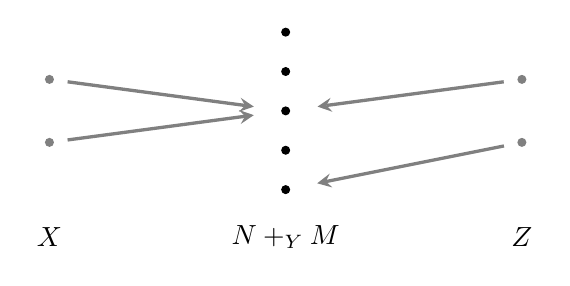
\begin{tikzpicture}[auto,scale=2]
    \node[circle,draw,inner sep=1pt,fill=gray,color=gray] (x1) at (1.5,.2) {};
    \node[circle,draw,inner sep=1pt,fill=gray,color=gray] (x2) at (1.5,-.2) {};
    \node at (1.5,-.8) {$X$};
    \node[circle,draw,inner sep=1pt,fill]         (A) at (3,.5) {};
    \node[circle,draw,inner sep=1pt,fill]         (B) at (3,.25) {};
    \node[circle,draw,inner sep=1pt,fill]         (C) at (3,0) {};
    \node[circle,draw,inner sep=1pt,fill]         (D) at (3,-.25) {};
    \node[circle,draw,inner sep=1pt,fill]         (E) at (3,-.5) {};
    \node at (3,-.8) {$N+_YM$};
    \node[circle,draw,inner sep=1pt,fill=gray,color=gray] (z1) at (4.5,.2) {};
    \node[circle,draw,inner sep=1pt,fill=gray,color=gray] (z2) at (4.5,-.2) {};
    \node at (4.5,-.8) {$Z$};
    \path[color=gray, very thick, shorten >=10pt, shorten <=5pt, ->, >=stealth]
    (x1) edge (C);
    \path[color=gray, very thick, shorten >=10pt, shorten <=5pt, ->, >=stealth]
    (x2) edge (C);
    \path[color=gray, very thick, shorten >=10pt, shorten <=5pt, ->, >=stealth]
    (z1) edge (C);
    \path[color=gray, very thick, shorten >=10pt, shorten <=5pt, ->, >=stealth]
    (z2) edge (E);
  \end{tikzpicture}
\end{center}
Here we see essentially the same phenomenon as we described for circuits above:
the apex of the cospan is much larger than the image of the maps from the feet.

Corelations address this with what is known as a $(\mc E,\mc M)$-factorisation
system. A factorisation system comprises subcategories $\mc E$ and $\mc M$ of
$\mc C$ such that every morphism in $\mc C$ factors, in a coherent way, as the
composite of a morphism in $\mc E$ followed by a morphism in $\mc M$. An
example, known as the epi-mono factorisation system on $\Set$, is yielded by the
observation that every function can be written as a surjection followed by an
injection.

Corelations, or more precisely $(\mc E,\mc M)$-corelations, are cospans $X
\to N \leftarrow Y$ such that the copairing $X+Y \to N$ of the two maps is an
element of the first factor $\mc E$ of the factorisation system. Composition of
corelations proceeds first as composition of cospans, but then takes only the
so-called $\mc E$-part of the composite cospan, to ensure the composite is again
a corelation. If we take the $\mc E$-part of a cospan $X \to N \leftarrow Y$, we
write the new apex $\overline{N}$, and so the resulting corelation $X \to
\overline{N} \leftarrow Y$. 

Mapping the above two cospans to epi-mono corelations in $\FinSet$ they become 
\begin{center}
  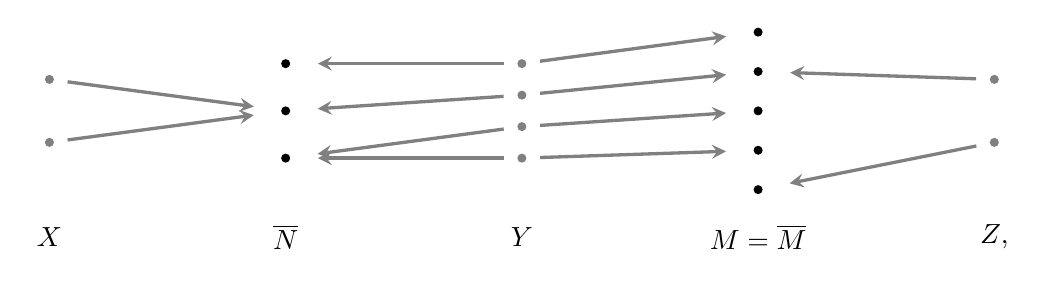
\begin{tikzpicture}[auto,scale=2]
    \node[circle,draw,inner sep=1pt,fill=gray,color=gray] (x1) at (-1.5,.2) {};
    \node[circle,draw,inner sep=1pt,fill=gray,color=gray] (x2) at (-1.5,-.2) {};
    \node at (-1.5,-.8) {$X$};
    \node[circle,draw,inner sep=1pt,fill]         (B) at (0,.3) {};
    \node[circle,draw,inner sep=1pt,fill]         (C) at (0,0) {};
    \node[circle,draw,inner sep=1pt,fill]         (D) at (0,-.3) {};
    \node at (0,-.8) {$\overline{N}$};
    \node[circle,draw,inner sep=1pt,fill=gray,color=gray] (y1) at (1.5,.3) {};
    \node[circle,draw,inner sep=1pt,fill=gray,color=gray] (y2) at (1.5,.1) {};
    \node[circle,draw,inner sep=1pt,fill=gray,color=gray] (y3) at (1.5,-.1) {};
    \node[circle,draw,inner sep=1pt,fill=gray,color=gray] (y4) at (1.5,-.3) {};
    \node at (1.5,-.8) {$Y$};
    \node[circle,draw,inner sep=1pt,fill]         (A') at (3,.5) {};
    \node[circle,draw,inner sep=1pt,fill]         (B') at (3,.25) {};
    \node[circle,draw,inner sep=1pt,fill]         (C') at (3,0) {};
    \node[circle,draw,inner sep=1pt,fill]         (D') at (3,-.25) {};
    \node[circle,draw,inner sep=1pt,fill]         (E') at (3,-.5) {};
    \node at (3,-.8) {$M=\overline{M}$};
    \node[circle,draw,inner sep=1pt,fill=gray,color=gray] (z1) at (4.5,.2) {};
    \node[circle,draw,inner sep=1pt,fill=gray,color=gray] (z2) at (4.5,-.2) {};
    \node at (4.5,-.8) {$Z$,};
    \path[color=gray, very thick, shorten >=10pt, shorten <=5pt, ->, >=stealth]
    (x1) edge (C);
    \path[color=gray, very thick, shorten >=10pt, shorten <=5pt, ->, >=stealth]
    (x2) edge (C);
    \path[color=gray, very thick, shorten >=10pt, shorten <=5pt, ->, >=stealth]
    (y1) edge (B);
    \path[color=gray, very thick, shorten >=10pt, shorten <=5pt, ->, >=stealth]
    (y2) edge (C);
    \path[color=gray, very thick, shorten >=10pt, shorten <=5pt, ->, >=stealth]
    (y3) edge (D);
    \path[color=gray, very thick, shorten >=10pt, shorten <=5pt, ->, >=stealth]
    (y4) edge (D);
    \path[color=gray, very thick, shorten >=10pt, shorten <=5pt, ->, >=stealth]
    (y1) edge (A');
    \path[color=gray, very thick, shorten >=10pt, shorten <=5pt, ->, >=stealth]
    (y2) edge (B');
    \path[color=gray, very thick, shorten >=10pt, shorten <=5pt, ->, >=stealth]
    (y3) edge (C');
    \path[color=gray, very thick, shorten >=10pt, shorten <=5pt, ->, >=stealth]
    (y4) edge (D');
    \path[color=gray, very thick, shorten >=10pt, shorten <=5pt, ->, >=stealth]
    (z1) edge (B');
    \path[color=gray, very thick, shorten >=10pt, shorten <=5pt, ->, >=stealth]
    (z2) edge (E');
  \end{tikzpicture}
\end{center}
with composite
\begin{center}
  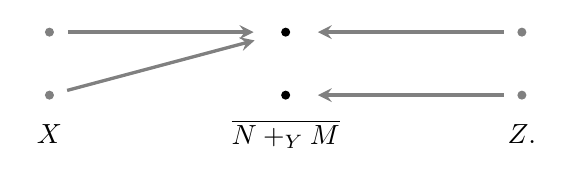
\begin{tikzpicture}[auto,scale=2]
    \node[circle,draw,inner sep=1pt,fill=gray,color=gray] (x1) at (1.5,.2) {};
    \node[circle,draw,inner sep=1pt,fill=gray,color=gray] (x2) at (1.5,-.2) {};
    \node at (1.5,-.45) {$X$};
    \node[circle,draw,inner sep=1pt,fill]         (A) at (3,.2) {};
    \node[circle,draw,inner sep=1pt,fill]         (B) at (3,-.2) {};
    \node at (3,-.45) {$\overline{N+_YM}$};
    \node[circle,draw,inner sep=1pt,fill=gray,color=gray] (z1) at (4.5,.2) {};
    \node[circle,draw,inner sep=1pt,fill=gray,color=gray] (z2) at (4.5,-.2) {};
    \node at (4.5,-.45) {$Z$.};
    \path[color=gray, very thick, shorten >=10pt, shorten <=5pt, ->, >=stealth]
    (x1) edge (A);
    \path[color=gray, very thick, shorten >=10pt, shorten <=5pt, ->, >=stealth]
    (x2) edge (A);
    \path[color=gray, very thick, shorten >=10pt, shorten <=5pt, ->, >=stealth]
    (z1) edge (A);
    \path[color=gray, very thick, shorten >=10pt, shorten <=5pt, ->, >=stealth]
    (z2) edge (B);
  \end{tikzpicture}
\end{center}
Note that the apex of the composite corelation is the subset of the apex of the
composite cospan comprising those elements that are in the image of the maps
from the feet. The intuition, again, is that composition of corelations discards
irrelevant information---of course, exactly what it discards depends on our
choice of factorisation system.

In this chapter we show that given a category $\mc C$ with finite colimits and a
factorisation system $(\mc E,\mc M)$, if $\mc M$ obeys a condition known as
`stability under pushout', then corelations in $\mc C$ form a hypergraph
category. We also show that given a colimit-preserving functor $A$ between such
categories $\mathcal C$, $\mathcal C'$ with factorisation systems $(\mathcal E,
\mathcal M)$, $(\mathcal E', \mathcal M')$, $A$ induces a hypergraph functor
between their corelation categories if the image of $\mathcal M$ lies in
$\mathcal M'$.

\section{Corelations} \label{sec.corels}

Given sets $X$, $Y$, a relation $X \to Y$ is a subset of the product $X
\times Y$. Note that by the universal property of the product, spans $X
\leftarrow N \to Y$ are in one-to-one correspondence with functions $N \to X
\times Y$. When this map is monic, we say that the span is \emph{jointly monic}.
More abstractly then, we might say a relation is an isomorphism class of jointly
monic spans in the category of sets. Here we generalise the dual concept: these
are our so-called corelations.

Relations and, equivalently, multi-valued functions have long been a structure
of mathematical interest, with their formalisation going back to De Morgan
\cite{DeM60} and Pierce \cite{Pie70} in the nineteenth century. One hundred
years later, their category theoretic generalisation as subobjects of pairwise
products was introduced by Puppe \cite{Pup62} and Mac Lane \cite{Mac63a} in the
setting of abelian categories, and Barr \cite{Bar70} for regular categories.
Subsequently, Klein \cite{Kle70} provided conditions under which these relations
can be given an associative composition rule---albeit conditions slightly more
restrictive than that which we use here---and by now the categorical theory of
relations is well studied \cite{FS90, Mil00, JW00}.  The key insight is the
definition of a factorisation system. We begin this section by introducing this
idea, before developing the theory of not just categories of relations, but
monoidal categories of (co)relations.

\subsection{Factorisation systems}
The relevant properties of jointly monic spans come from the fact that
monomorphisms form one half of a factorisation system. A factorisation system
allows any morphism in a category to be factored into the composite of two
morphisms in a coherent way. This subsection introduces factorisation systems
and monoidal factorisation systems.

\begin{definition}
  A \define{factorisation system} $(\mathcal E,\mathcal M)$ in a category
  $\mathcal C$ comprises subcategories $\mathcal E$, $\mathcal M$ of $\mathcal
  C$ such that
  \begin{enumerate}[(i)]
    \item $\mathcal E$ and $\mathcal M$ contain all isomorphisms of $\mathcal
      C$.
    \item  every morphism $f \in \mathcal C$ admits a factorisation $f=m \circ
      e$, $e \in \mathcal E$, $m \in \mathcal M$.
\item given morphisms $f,f'$, with factorisations $f = m \circ e$, $f' = m' \circ
  e'$ of the above sort, for every $u$, $v$ such that the square
  \[
    \xymatrixcolsep{3pc}
    \xymatrixrowsep{3pc}
    \xymatrix{
       \ar[r]^f \ar[d]_u &  \ar[d]^v \\
       \ar[r]_{f'} & 
    }
  \]
  commutes, there exists a unique morphism $s$ such that
  \[
    \xymatrixcolsep{3pc}
    \xymatrixrowsep{3pc}
    \xymatrix{
      \ar[r]^e \ar[d]_u & \ar[r]^m \ar@{.>}[d]^{\exists! s} &  \ar[d]^v \\
       \ar[r]_{e'}& \ar[r]_{m'} & 
    }
  \]
  commutes.
  \end{enumerate}
\end{definition}

\begin{examples} \label{ex.factsysts}\ 

  \begin{itemize}
    \item Write $\mathcal I_{\mathcal C}$ for the wide subcategory of
      $\mathcal C$ containing exactly the isomorphisms of $\mathcal C$. Then
      $(\mathcal I_{\mathcal C}, \mathcal C)$ and $(\mathcal C, \mathcal
      I_{\mathcal C})$ are both factorisation systems in $\mathcal C$. While
      these may seem too trivial to mention, we will see they are of central
      importance in what follows.
    
    \item The prototypical example of a factorisation system is the epi-mono
      factorisation system $(\mathrm{Sur},\mathrm{Inj})$ in $\Set$. Here we
      write $\mathrm{Sur}$ for the subcategory of surjections in $\Set$, and
      $\mathrm{Inj}$ for the subcategory of injections. 
      
      Recall that a split monomorphism is a map $m\colon X\to Y$ such that there
      exists a one-sided inverse, i.e. a map $m'\colon Y\to X$ such that
      $m'm=\idn_X$. Observe that, assuming the axiom of choice, all monos in
      $\Set$ split.  One way of proving that the above is a factorisation system
      on $\Set$ is via the more general fact, true in any category: if every
      arrow can be factorised as an epi followed by a split mono, then
      epimorphisms and split monomorphisms form the factors of a factorisation
      system.  The only non-trivial part to check is the uniqueness condition:
      given epis $e_1,e_2$, split monos $m_1,m_2$, and commutative diagram
      \[
	\xymatrixcolsep{3pc}
	\xymatrixrowsep{3pc}
	\xymatrix{
	  \ar[r]^{e_1} \ar[d]_u & \ar[r]^{m_1} \ar@{.>}[d]^{\exists! t} &
	  \ar[d]^v \\
	  \ar[r]_{e_2}& \ar[r]_{m_2} & 
	}
      \]
      we must show that there is a unique $t$ that makes the diagram commute.
      Indeed let $t= m_2'vm_1$ where $m_2'$ satisfies $m_2'm_2=id$. 
      To see that the right square commutes, observe
      \[
	m_2 t e_1 =  m_2 m_2' v m_1 e_1 = m_2 m_2' m_2 e_2 u = m_2 e_2 u = v m_1 e_1
      \]
      and since $e_1$ is epi we have $m_2 t = v m_1$. For the left square,
      \[
	t e_1 = m_2' v m_1 e_1 = m_2' m_2 e_2 u = e_2 u.
      \] 
      Uniqueness is immediate, since, $e_1$ is epi and $m_2$ is mono. 
    
    \item Recall that a regular epimorphism is an epimorphism that is the
      coequaliser for some pair of parallel morphisms. (Dually, a regular
      monomorphism is an equaliser for some pair of parallel morphisms.) In any
      so-called regular category the regular epimorphisms and monomorphisms form
      a factorisation system.  Examples of regular categories include $\Set$,
      toposes, and abelian categories. Regular categories were introduced by
      Barr and Grillet; for more details see \cite{Bar71,Gri71}.
\end{itemize}
More details and further examples can be found in \cite[\textsection 14]{AHS}.
\end{examples}

As we are concerned with building monoidal categories of corelations, it will be
important that our factorisation systems are monoidal factorisation systems.

\begin{definition}
Call a factorisation system $(\mc E,\mc M)$ in a monoidal category $(\mc C,\ot)$
a \define{monoidal factorisation system} if $(\mc E,\ot)$ is a monoidal
category.
\end{definition}

One might wonder why $\mc M$ does not appear in the above definition. To give a
touch more intuition for this definition, we quote a theorem of Ambler. Recall a
symmetric monoidal closed category is one in which each functor $- \ot X$ has a
specified right adjoint $[X,-]$. 
\begin{proposition}
  Let $(\mc E,\mc M)$ be a factorisation system in a symmetric monoidal
  closed category $(\mc C,\ot)$. Then the following are equivalent:
  \begin{enumerate}[(i)]
    \item $(\mc E,\mc M)$ is a monoidal factorisation system.
    \item $\mc E$ is closed under $- \ot X$ for all $X \in \mc C$.
    \item $\mc M$ is closed under $[X,-]$ for all $X \in \mc C$.
\end{enumerate}
\end{proposition}
\begin{proof}
  See Ambler for proof and further details \cite[Lemma 5.2.2]{Am}.
\end{proof}


We need not worry too much, however, about the distinction between factorisation
systems and monoidal factorisation systems. The reason is that for our
purposes---where the underlying category $\mc C$ has finite colimits and the
monoidal product is the coproduct---\emph{all} factorisation systems are
monoidal factorisation systems. This is implied by the following lemma.

\begin{lemma} \label{lem.monfact}
  Let $\mc C$ be a category with finite coproducts, and let $(\mc E, \mc M)$ be a
  factorisation system on $\mc C$. Then $(\mc E,+)$ is a symmetric monoidal
  category.
\end{lemma}
\begin{proof}
  The only thing to check is that $\mc E$ is closed under $+$. That is, given
  $f\maps A \to B$ and $g\maps C \to D$ in $\mc E$, we wish to show that
  $f+g\maps A+C \to B+D$, defined in $\mc C$, is also a morphism in $\mc E$. 

  Let $f+g$ have factorisation $A+C \stackrel{e}\longrightarrow \overline{B+D}
  \stackrel{m}\longrightarrow B+D$, where $e \in \mc E$ and $m \in \mc
  M$. We will prove that $m$ is an isomorphism. To construct an inverse, recall
  that by definition, as $f$ and $g$ lie in $\mc E$, there exist morphisms
  $x\maps B \to \overline{B+D}$ and $y\maps D \to \overline{B+D}$ such that
  \[ \label{eq.coreltensor}
    \xymatrixcolsep{2pc}
    \xymatrixrowsep{2pc}
    \xymatrix{
      A \ar[r]^f \ar[d] & B \ar@{=}[r] \ar@{.>}[d]^x & B
      \ar[d] \\
      A+C \ar[r]_{e}&\overline{B+D} \ar[r]_{m} & B+D
    }
    \qquad \mbox{and} \qquad
    \xymatrixcolsep{2pc}
    \xymatrixrowsep{2pc}
    \xymatrix{
      C \ar[r]^g \ar[d] & D \ar@{=}[r] \ar@{.>}[d]^y & D
      \ar[d] \\
      A+C \ar[r]_{e}&\overline{B+D} \ar[r]_{m} & B+D
    }
    \tag{1}
  \]
  The copairing $[x,y]$ is an inverse to $m$. 
  
  Indeed, taking the coproduct of the top rows of the two diagrams above and the
  copairings of the vertical maps gives the commutative diagram
  \[
    \xymatrix{
      A+C \ar[r]^{f+g} \ar@{=}[d] & B+D \ar@{=}[r] \ar[d]_{[x,y]} & B+D \ar@{=}[d] \\
      A+C \ar[r]^{e} & \overline{B+D} \ar[r]^{m} & B+D
    }
  \]
  Reading the right-hand square immediately gives $m \circ [x,y] =1$.
  
  Conversely, to see that $[x,y] \circ m = 1$, remember that by definition $f+g
  = m \circ e$. So the left-hand square above implies that
  \[
    \xymatrixcolsep{2pc}
    \xymatrixrowsep{2pc}
    \xymatrix{
      A+C \ar[r]^e \ar@{=}[d] & \overline{B+D} \ar[d]^{[x,y] \circ m} \\
      A+C \ar[r]_{e}&\overline{B+D} 
    }
  \]
  commutes. But by the universal property of factorisation systems, there is a
  unique map $\overline{B+D} \to \overline{B+D}$ such that this diagram
  commutes, and clearly the identity map also suffices. Thus $[x,y] \circ m =
  1$.
\end{proof}

\subsection{Corelations}
Now that we have introduced factorisation systems, observe that relations are
just spans $X \leftarrow N \to Y$ in $\Set$ such that $N \to X \times Y$ is an
element of $\mathrm{Inj}$, the right factor in the factorisation system
$(\mathrm{Sur},\mathrm{Inj})$. Relations may thus be generalised as spans such
that the span maps jointly belong to some class $\mc M$ of an $(\mc E,\mc
M)$-factorisation system. We define corelations in the dual manner.

\begin{definition}
  Let $\mathcal C$ be a category with finite colimits, and let $(\mathcal E,
  \mathcal M)$ be a factorisation system on $\mathcal C$. An $(\mathcal
  E,\mathcal M)$\define{-corelation} $X \to Y$ is a cospan $X
  \stackrel{i}\longrightarrow N \stackrel{o}\longleftarrow Y$ in $\mc C$ such
  that the copairing $[i,o]\maps X+Y \to N$ lies in $\mathcal E$.
\end{definition}

When the factorisation system is clear from context, we simply call $(\mathcal
E,\mathcal M)$-corelations `corelations'.

We also say that a cospan $X \stackrel{i}\longrightarrow N
\stackrel{o}\longleftarrow Y$ with the property that the copairing $[i,o]\maps
X+Y \to N$ lies in $\mathcal E$ is \define{jointly} $\mathcal E$\define{-like}.
Note that if a cospan is jointly $\mc E$-like then so are all isomorphic
cospans. Thus the property of being a corelation is closed under isomorphism of
cospans, and we again are often lazy with our language, referring to both
jointly $\mc E$-like cospans and their isomorphism classes as corelations. 

If $f\maps A \to N$ is a morphism with factorisation $f = m \circ e$, write
$\overline N$ for the object such that $e\maps A \to \overline N$ and $m\maps
\overline N \to N$. Now, given a cospan $X \stackrel{i_X}{\longrightarrow} N
\stackrel{o_Y}{\longleftarrow} Y$, we may use the factorisation system to write
the copairing $[i_X,o_Y]\maps X+Y \to N$ as
\[
  X+Y \stackrel{e}{\longrightarrow} \overline{N} \stackrel{m}{\longrightarrow}
  N.
\]
From the universal property of the coproduct, we also have maps $\iota_X\maps X
\to X+Y$ and $\iota_Y\maps Y \to X+Y$. We then call the corelation 
\[
  X \stackrel{e\circ \iota_X}{\longrightarrow} \overline{N} \stackrel{e \circ
  \iota_Y}{\longleftarrow} Y
\]
the $\mathcal E$\define{-part} of the above cospan. On occasion we will also
write $e\maps X+Y \to \overline N$ for the same corelation.

\begin{examples} \label{ex.corels}
  Many examples of corelations are already familiar.
  \begin{itemize}
    \item For the morphism-isomorphism factorisation system $(\mc C,\mc I_{\mc
      C})$, corelations are just cospans.

    \item For the isomorphism-morphism factorisation $(\mc I_{\mc C}, \mc C)$,
      jointly $\mc I_{\mc C}$-like cospans $X \to Y$ are simply isomorphisms
      $X+Y \stackrel\sim\to N$. Thus there is a unique isomorphism class of
      corelations between any two objects.

    \item Note that the category $\Set$ has finite colimits and an epi-mono
      factorisation system $(\mathrm{Sur},\mathrm{Inj})$. Epi-mono corelations
      from $X \to Y$ in $\mathrm{Set}$ are surjective functions $X+Y \to N$;
      thus their isomorphism classes are partitions, or equivalence relations on
      $X+Y$. 

      While this compositional structure on equivalence relations has not the
      prominence of that on relations, these corelations have been recognised as
      an important structure. Ellerman gives a detailed treatment from a logic
      viewpoint in \cite{Ell14}, while basic category theoretic aspects can be
      found in Lawvere and Rosebrugh \cite{LR}.  Note that in these and in other
      sources, including \cite{CF,BF}, the term corelation is used to solely
      refer to these $(\mathrm{Sur},\mathrm{Inj})$-corelations in $\Set$, while
      here we use the term corelation primarily in the generalised sense.
  \end{itemize}
\end{examples}

Our next task is to define a composition rule on corelations.

\subsection{Categories of corelations} \label{ssec.corelcats}
We begin this subsection by defining a composition rule on isomorphism classes
of corelations. The end goal, however, is to define a hypergraph category in
which the morphism are corelations. Here we will explain how to define such a
category, introducing and exploring the important condition that $\mc M$ is
stable under pushout. We leave the proof that we have truly defined a hypergraph
category for the next subsection.

We compose corelations by taking the $\mathcal E$-part of their composite
cospan. That is, given corelations $X \stackrel{i_X}{\longrightarrow} N
\stackrel{o_Y}{\longleftarrow} Y$ and $Y \stackrel{i_Y}{\longrightarrow} M
\stackrel{o_Z}{\longleftarrow} Z$, their composite is given by the cospan $X
\xrightarrow{e\circ\iota_X} \overline{N+_YM} \xleftarrow{e \circ \iota_Z} Z$ in the commutative diagram
\[
  \begin{tikzcd}[row sep=7ex,column sep=7ex]
    && N+_YM \\
    && \overline{N+_YM} \arrow[u,pos=.4,"m"] \\
    & N \arrow[uur,"j_N"] & X+Z \arrow[from=dll,pos=.35,swap,"\iota_X"]
    \arrow[from=drr,pos=.35,"\iota_Z"]
    \arrow[u,"e"] & 
    M \arrow[uul,swap,"j_M"] \\
    X \arrow[ur,"i_X"] && Y
    \arrow[ul,crossing over,pos=.35,"o_Y"] \arrow[ur,crossing
    over,pos=.35,swap,"i_Y"] && Z,
    \arrow[ul,swap,"o_Z"]
  \end{tikzcd}
\]
where $m \circ e$ is the $(\mc E,\mc M)$-factorisation of $[j_N\circ i_X,j_M
\circ o_Z]\maps X+Z
\to N+_YM$. 

It is well known that this composite is unique up to isomorphism, and that when
$\mc M$ is well behaved it defines a category with isomorphism classes of
corelations as morphisms. For instance, a bicategorical version of the dual
theorem, for spans and relations, can be found in \cite{JW00}. Nonetheless, for
the sake of completeness we will explain all the details and sketch our own
argument here. The first fact to show is that, as we have just stated, the
composite of corelations is unique up to isomorphism.

\begin{proposition} \label{prop.corelcomp}
  Let $\mc C$ be a category with finite colimits and with a factorisation system
  $(\mc E,\mc M)$. Then the above is a well-defined composition rule on
  isomorphism classes of corelations.
\end{proposition}
\begin{proof}
  Let
  $(X \stackrel{i_X}{\longrightarrow} N \stackrel{o_Y}{\longleftarrow} Y$,
  $X \stackrel{i_X'}{\longrightarrow} N' \stackrel{o_Y'}{\longleftarrow} Y)$
%  \[
%    X \stackrel{i_X}{\longrightarrow} N \stackrel{o_Y}{\longleftarrow} Y 
%    \qquad \mbox{and} \qquad 
%    X \stackrel{i_X'}{\longrightarrow} N' \stackrel{o_Y'}{\longleftarrow} Y
%  \]
  and
  $(Y \stackrel{i_Y}{\longrightarrow} M \stackrel{o_Z}{\longleftarrow} Z$, $Y
  \stackrel{i_Y'}{\longrightarrow} M' \stackrel{o_Z'}{\longleftarrow} Z)$
%  \[
%    Y \stackrel{i_Y}{\longrightarrow} M \stackrel{o_Z}{\longleftarrow} Z 
%    \qquad \mbox{and} \qquad 
%    Y \stackrel{i_Y'}{\longrightarrow} M' \stackrel{o_Z'}{\longleftarrow} Z
%  \]
  be pairs of isomorphic jointly $\mathcal E$-like cospans. By Proposition
  \ref{prop.composingdeccospans} their composites \emph{as cospans} 
  % $(X \longrightarrow N+_YM \longleftarrow Z)$ and $(X
  %\longrightarrow N'+_YM' \longleftarrow Z)$
%  \[
%    X \longrightarrow N+_YM \longleftarrow Z 
%    \qquad \mbox{and} \qquad 
%    X \longrightarrow N'+_YM' \longleftarrow Z
%  \]
  are isomorphic via an isomorphism $p\maps N+_YM \to N'+_YM'$. The
  factorisation system then gives an isomorphism $s$ such that the diagram
  \[
    \xymatrixcolsep{3pc}
    \xymatrixrowsep{2pc}
    \xymatrix{
      X+Z \ar[r]^e \ar@{=}[d] & \overline{N+_YM} \ar[r]^m \ar@{.>}[d]^{s}_\sim & N+_YM
      \ar[d]_\sim^{p} \\
      X+Z \ar[r]_{e'}&\overline{N'+_YM'} \ar[r]_{m'} & N'+_YM'
    }
  \]
  commutes. Thus $s$ is an isomorphism of the composite corelations.
\end{proof}

As we have said, this composition rule only gives a category when $\mc M$ is
well behaved. The reason is that composition of corelations is \emph{not}
associative in general. It is, however, associative when $\mathcal M$ is stable
under pushout. We now define this, provide some examples, and prove a crucial
lemma.

\begin{definition}
  Given a category $\mc C$, we say that a subcategory $\mc M$ is \define{stable
  under pushout} if for every pushout square
  \[
    \xymatrixcolsep{3pc}
    \xymatrixrowsep{3pc}
    \xymatrix{
      \ar[r]^j & \\
      \ar[u] \ar[r]^m &  \ar[u]
    }
  \]
  such that $m \in \mathcal M$, we also have that $j \in \mathcal M$. 
\end{definition}

\begin{examples}
  There are many examples of $(\mc E,\mc M)$-factorisation systems with $\mc M$
  stable under pushout, including the factorisation systems $(\mc I_{\mc C},\mc
  C)$ and $(\mc C,\mc I_{\mc C})$ in $\mc C$, and $(\mathrm{Sur},\mathrm{Inj})$
  in $\Set$.

  This last example generalises to any topos. Indeed, Lack and Soboci\'nski
  showed that monomorphisms are stable under pushout in any adhesive category
  \cite{LS04}.  Since any topos is both a regular category and an adhesive
  category \cite{LS06,Lac11}, the regular epimorphism-monomorphism factorisation
  system in any topos is an $(\mc E,\mc M)$-factorisation system with $\mc M$
  stable under pushout.
  
  Another example is the dual of any regular category. Such a category is known
  as a coregular category, and is by definition a category that has finite
  colimits and an epimorphism-regular monomorphism factorisation system with
  regular monomorphisms stable under pushout. Examples of these include the
  category of topological spaces and continuous maps, as well as $\Set^\opp$,
  any cotopos, and so on.
\end{examples}

Stability under pushout is a powerful property. A key corollary, both for
associativity and in general, is that it implies $\mc M$ is also closed under
$+$. 
%For our proof sketch we rely on the following useful lemma.

\begin{lemma} \label{lem.mcoproductsmc}
  Let $\mathcal C$ be a category with finite colimits, and let $\mathcal M$ be a
  subcategory of $\mathcal C$ stable under pushouts and containing all
  isomorphisms. Then $(\mc M,+)$ is a symmetric monoidal category.
\end{lemma}
\begin{proof}
  It is enough to show that for all morphisms $m,m' \in \mc M$ we have $m+m'$ in
  $\mc M$. Since $\mc M$ contains all isomorphisms, the coherence maps are
  inherited from $\mc C$. The required axioms---the functoriality of the tensor
  product, the naturality of the coherence maps, and the coherence laws---are
  also inherited as they hold in $\mc C$.

  To see $m+m'$ is in $\mc M$, simply observe that we have the pushout square
  \[
  \xymatrixcolsep{3pc}
  \xymatrixrowsep{2pc}
    \xymatrix{
      A+C \ar[r]^{m+1} & B+C \\
      A \ar[r]^m \ar[u]^{\iota} & B \ar[u]_{\iota} \\
    }
  \]
  in $\mc C$. As $\mc M$ is stable under pushout, $m+1 \in \mc M$. Similarly,
  $1+m' \in \mc M$. Thus their composite $m+m'$ lies in $\mc M$, as required.
\end{proof}

An analogous argument shows that pushouts of maps $m+_Ym'$ also lie in $\mc M$.
Using this lemma it is not difficult to show associativity---the key point is
that factorisation `commutes' with pushouts, and that we have a category
$\corel_{(\mc E,\mc M)}(\mc C)$. Again, this is all well known, and can be found
in \cite{JW00}. We will incidentally reprove these facts in the following,
while pursuing richer structure.

%\begin{proposition}
%  Let $\mc C$ be a category with finite colimits and a factorisation system
%  $(\mc E,\mc M)$ such that $\mc M$ is stable under pushouts. Then composition
%  of corelations is associative.
%\end{proposition}
%\begin{proof}[Proof (sketch)]
%  The key concern is whether factorisation `commutes' with taking pushouts.
%  Using the above lemma and the fact that $\mc M$ is stable under pushouts, the
%  pushout square 
%  \[
%  \xymatrixcolsep{3pc}
%  \xymatrixrowsep{2pc}
%  \xymatrix{
%    N+_Y\overline{M} \ar[r]^{m'} & N+_YM \\
%    N+\overline{M} \ar[u] \ar[r]^{1+m} & N+M  \ar[u]
%  }
%  \]
%  shows that the map $m'\maps N+_Y\overline{M} \to N+_YM$ is in $\mc M$
%  whenever $m\maps \overline{N} \to N$ is. It can then be shown that the
%  composite of any number of corelations can be given by taking the composite of
%  them all as cospans, and then taking the jointly $\mc E$-like part.
%\end{proof}

%The identity axioms for corelations are self-evident. We thus have a category
%$\corel_{(\mc E,\mc M)}(\mc C)$.  Again, we will drop explicit reference to the
%factorisation system when context allows, simply writing $\mathrm{Corel}(\mc
%C)$.
%
%\begin{remark}
%An aside: proving associativity is not logically necessary in the development
%of this chapter. Associativity will follow from the existence of the functor
%from $\cospan(\mc C)$ to $\corel(\mc C)$, like the other necessary coherence
%results for hypergraph categories. Nonetheless, it is terminologically easier to
%establish that $\corel(\mc C)$ is indeed a category at this point, before we
%define hypergraph structure and functors on it.
%\end{remark}
%

Indeed, for modelling networks, we require not just a category, but a hypergraph
category. Corelation categories come equipped with this extra structure.  Recall
that we gave decorated cospan categories a hypergraph structure by defining a
wide embedding $\mathrm{Cospan}(\mc C) \hookrightarrow F\mathrm{Cospan}$, via
which $F\mathrm{Cospan}$ inherited the coherence and Frobenius maps (Theorem
\ref{thm:fcospans}). We will argue similarly here, after showing that the map
\[
  \cospan(\mc C) \longrightarrow \corel(\mc C)
\]
taking each cospan to its jointly $\mc E$-like part is functorial. Indeed, we
define the coherence and Frobenius maps of $\corel(\mc C)$ to be their image
under this map. For the monoidal product we again use the coproduct in $\mc C$;
the monoidal product of two corelations is their monoidal product as cospans.

\begin{theorem} \label{thm.cospantocorel}
  Let $\mathcal C$ be a category with finite colimits, and let $(\mathcal E,
  \mathcal M)$ be a factorisation system on $\mathcal C$ such that $\mathcal M$
  is stable under pushout. Then there exists a hypergraph category
  $\mathrm{Corel}_{(\mc E,\mc M)}(\mathcal C)$ with 
  \smallskip

  \begin{center}
    \begin{tabular}{| c | p{.65\textwidth} |}
      \hline
      \multicolumn{2}{|c|}{The hypergraph category $(\mathrm{Corel}_{(\mc E,\mc M)}(\mc C),+)$} \\
      \hline
      \textbf{objects} & the objects of $\mathcal C$ \\ 
      \textbf{morphisms} & isomorphism classes of $(\mc E,\mc M)$-corelations in $\mathcal C$\\ 
      \textbf{composition} & given by the $\mc E$-part of pushout \\
      \textbf{monoidal product} & the coproduct in $\mathcal C$ \\
      \textbf{coherence maps} & inherited from $\cospan(\mc C)$  \\
      \textbf{hypergraph maps} & inherited from $\cospan(\mc C)$ \\
      \hline
    \end{tabular}
  \end{center}  
  \smallskip
\end{theorem}

Again, we will drop explicit reference to the factorisation system when context allows, simply writing $\mathrm{Corel}(\mc C)$.

\begin{examples} \label{ex.corelcats}
In each factorisation system of Examples \ref{ex.corels} the right factor
$\mathcal M$ is stable under pushout. The hypergraph category 
$\corel_{(\mc C,\mc I_{\mc C})}(\mc C)$ is just the hypergraph category of
cospans in $\mc C$. In the hypergraph category $\corel_{(\mc I_{\mc C},\mc
C)}(\mc C)$, the only morphism between any two objects $X$ and $Y$ is the
isomorphism class of the corelation $X \xrightarrow{\iota_X} X+Y
\xleftarrow{\iota_Y} Y$ corresponding to the identity map $X+Y \to X+Y$ in $\mc
I_{\mc C}$. Thus $\corel_{(\mc I_{\mc C},\mc C)}(\mc C)$ is the indiscrete
category on the objects of $\mc C$. 

We discussed epi-mono corelations in $\FinSet$ informally in our motivation
section \textsection\ref{sec.blackboxing}. These are equivalence relations
between finite sets. This example is perhaps the most instructive for
black-boxing open systems, and we will return to it in
\textsection\ref{ssec.equivrels}.
\end{examples}

Proposition \ref{prop.corelcomp} shows that our composition rule is a
well-defined function; Lemma \ref{lem.monfact} shows likewise for the monoidal
product $+\maps \corel(\mc C)\times \corel(\mc C) \to \corel(\mc C)$. Thus we
have the required data for a hypergraph category. It remains to check a
number of axioms: associativity and unitality of the categorical composition,
functoriality of the monoidal product, naturality of the coherence maps, the
coherence axioms for symmetric monoidal categories, the Frobenius laws.

Our strategy for this will be to show that the surjective function from cospans
to corelations defined by taking a cospan to its jointly $\mc E$-part preserves
both composition and the monoidal product. This then implies that to evaluate an
expression in the monoidal category of corelations, we may simply evaluate it in
the monoidal category of cospans, and then take the $\mc E$-part. Thus if an
equation is true for cospans, it is true for corelations.

Instead of proving just this, however, we will prove a generalisation regarding
an analogous map between any two corelation categories. Such a map exists
whenever we have two corelation categories $\corel_{(\mc E,\mc M)}(\mc C)$ and
$\corel_{(\mc E',\mc M')}(\mc C')$ and a colimit
preserving functor $A\maps \mc C \to \mc C'$ such that the image of $\mc M$ lies
in $\mc M'$. As $(\mc C,\mc I_{\mc C})$-corelations are just cospans, this
reduces to the desired special case by taking the domain to be the category of
$(\mc C,\mc I_{\mc C})$-corelations, $\mc C'$ to be equal to $\mc C$, and $A$ to
be the identity functor. But the generality is not spurious: it has the
advantage of proving the existence of a class of hypergraph functors between
corelation categories in the same fell swoop.

Although a touch convoluted, this strategy is worth the pause for thought. We
will use it once again for \emph{decorated} corelations, to great economy.

%\begin{lemma}
%  The map $(-)+(-)\maps \corel(\mc C)\times\corel(\mc C) \to \corel(\mc C)$
%  induced by the coproduct in $\mc C$ is functorial.
%\end{lemma}
%\begin{proof}
%As a preliminary, note that $+$ is a well-defined function: Lemma
%\ref{lem.monfact} implies that the coproduct of two corelations is again a
%corelation. Our task is to show that, given the four corelations 
%\[
%  \xymatrixrowsep{0pt}
%  \xymatrix{
%  f= X \longrightarrow N \longleftarrow Y  & &
%  g= Y \longrightarrow M \longleftarrow Z \\
%  h = X' \longrightarrow N' \longleftarrow Y' & &
% k= Y' \longrightarrow M' \longleftarrow Z'
%}
%\]
%we have $(g \circ f) + (k \circ h) = (g + k) \circ (f + h)$. The left and
%right side of this expression are respectively given by the first arrow in the
%upper and lower rows of the commutative diagram
%\[
%  \xymatrix{
%    (X+Z)+(X'+Z') \ar[r]^{\mc E+\mc E} \ar[d]^{\sim} & 
%    (\overline{N+_YM})+(\overline{N'+_{Y'}M'}) \ar[r]^{\mc M+\mc M} \ar@{.}[d] &
%    (N+_YM)+(N'+_{Y'}M') \ar[d]^{\sim} \\
%    (X+X')+(Z+Z') \ar[r]^{\mc E} &
%    \overline{(N+N')+_{Y+Y'}(M+M')} \ar[r]^{\mc M} & 
%    (N+N')+_{Y+Y'}(M+M'). \\
%  }
%\]
%The leftmost and rightmost vertical arrows are isomorphisms by properties of
%colimits. The upper row is an $(\mc E,\mc M)$-factorisation as the first map is
%the coproduct of two maps in $\mc E$ and the second map is the coproduct of two
%maps in $\mc M$, both of which are monoidal with respect to the coproduct
%(Lemmas \ref{lem.monfact} and \ref{lem.mcoproductsmc}). The lower row is an
%$(\mc E,\mc M)$-factorisation by definition. Thus, by the properties of
%factorisation systems, the dotted map $s$ is an isomorphism, and hence $+$ is
%functorial. 
%\end{proof}
%
%To prove Theorem \ref{thm.cospantocorel} it remains to show that our proposed
%data for $\mathrm{Corel}(\mc C)$ obey the necessary axioms: the symmetric
%monoidal coherence laws, the special commutative Frobenius monoid laws. Our
%proof strategy will be a touch complicated. Again, recall that in Theorem
%\ref{thm:fcospans} we proved $F\mathrm{Cospan}$ had hypergraph structure via
%a functor from $\cospan(\mc C)$. Instead of proving each axiom directly, we will
%again leverage the fact that we already know $\cospan(\mc C)$ is a hypergraph
%category, and show that $\corel(\mc C)$ is the image of $\cospan(\mc C)$ under a
%composition-preserving map that also respects (indeed, defines) the monoidal and
%hypergraph structure.
%
%Note that $\mc C$ is trivially stable under pushout. By definition we have the
%equality of hypergraph categories $\mathrm{Corel}_{(\mc C,\mc I_{\mc C})}(\mc
%C)= \cospan(\mc C)$. Thus the functor $\cospan(\mc C) \to \mathrm{Corel}(\mc C)$
%is a special case of functors between corelation categories. Taking advantage of
%this, we will discuss functors between corelation categories in general, before
%specialising to this case to prove that $\mathrm{Corel}(\mc C)$ indeed is a
%well-defined hypergraph category.
%
%This will be done in the next subsection.



\section{Functors between corelation categories} \label{sec.corelfunctors}
We have seen that to construct a functor between cospan categories one may start
with a colimit-preserving functor between the underlying categories. Corelations
are cospans where we forget the $\mc M$-part of each cospan. Hence for functors
between corelation categories, we require not just a colimit-preserving functor
but, loosely speaking, also that we don't forget too much in the domain category
compared to the codomain category.

We devote the next few pages to proving the following proposition. Along the way
we prove, as promised, that corelation categories are well-defined hypergraph
categories.

\begin{proposition} \label{prop.corelfunctors}
  Let $\mathcal C$, $\mathcal C'$ have finite colimits and respective
  factorisation systems $(\mathcal E, \mathcal M)$, $(\mathcal E', \mathcal M')$,
  such that $\mathcal M$ and $\mathcal M'$ are stable under pushout. Further let
  $A\maps \mathcal C \to \mathcal C'$ be a functor that preserves finite colimits
  and such that the image of $\mathcal M$ lies in $\mathcal M'$.

  Then we may define a hypergraph functor $\square\maps \corel(\mathcal C) \to
  \corel(\mathcal C')$ sending each object $X$ in $\corel(\mathcal C)$ to $AX$ in
  $\corel(\mc C')$ and each corelation 
  \[
    X \stackrel{i_X}{\longrightarrow} N \stackrel{o_Y}{\longleftarrow} Y 
  \]
  to the $\mc E'$-part
  \[
    AX \xrightarrow{e'\circ\iota_{AX}} \overline{AN}
    \xleftarrow{e'\circ\iota_{AY}} AY.
  \]
  of the image cospan. The coherence maps are the $\mc E'$-part
  $\overline{\kappa_{X,Y}}$ of the isomorphisms $\kappa_{X,Y}\maps AX+AY \to
  A(X+Y)$ given as $A$ preserves colimits.
\end{proposition}

As discussed, we still have to prove that $\corel(\mc C)$ is a hypergraph
category. We address this first with two lemmas regarding these proposed
functors.

\begin{lemma} \label{lem.corelfuncomposition}
  The above function $\square\maps \corel(\mc C) \to \corel(\mc C')$ preserves
  composition.
\end{lemma}
\begin{proof}
  Let $f = (X \longrightarrow N \longleftarrow Y)$ and $g= (Y \longrightarrow M
  \longleftarrow Z)$ be corelations in $\mathcal C$. By definition, the
  corelations $\square(g) \circ \square(f)$ and $\square(g \circ f)$ are given
  by the first arrows in the top and bottom row respectively of the diagram:
  \[ \label{diag.eparts}
    \begin{aligned}
      \xymatrixcolsep{5.5pc}
      \xymatrixrowsep{2pc}
      \xymatrix{
	\scriptstyle AX+AZ \ar[r]^{\mc E'} \ar@{=}[d] & \scriptstyle \overline{\overline{AN}+_{AY}\overline{AM}}
	\ar[r]^{\mc M'} \ar@{<.>}[d]^{n} & \scriptstyle \overline{AN}+_{AY}\overline{AM}
	\ar[r]^{m'_{AN}+_{AY}m'_{AM}} & \scriptstyle
	AN+_{AY}AM \\
	\scriptstyle AX+AZ \ar[r]^{\mc E'} & \scriptstyle \overline{A(\overline{N+_YM})} \ar[r]^{\mc M'} & \scriptstyle
	A(\overline{N+_YM}) \ar[r]^{Am_{N+_YM}} & \scriptstyle A(N+_YM) \ar@{<->}[u]_{\sim}
      }
    \end{aligned}
    \tag{$\ast$}
  \]
  The morphisms labelled $\mc E'$ lie in $\mc E'$, and similarly for $\mc M'$;
  these are given by the factorisation system on $\mc C'$.  The maps
  $Am_{N+_YM}$ and $m'_{AN}+_{AY}m'_{AM}$ lie in $\mc M'$ too: $Am_{N+_YM}$ as
  it is in the image of $\mc M$, and $m'_{AN}+_{AY}m'_{AM}$ as $\mc M'$ is
  stable under pushout. 

  Moreover, the diagram commutes as both maps $AX+AZ \to AN+_{AY}AM$ compose to
  that given by the pushout of the images of $f$ and $g$ over $AY$.  Thus the
  diagram represents two $(\mc E', \mc M')$ factorisations of the same morphism,
  and there exists an isomorphism $n$ between the corelations $\square(g) \circ
  \square(f)$ and $\square(g\circ f)$. This proves that $\square$ preserves
  composition.
\end{proof}
This first lemma allows us to verify the associativity and unit laws for
$\corel(\mc C)$.
\begin{corollary}
  $\corel(\mc C)$ is well defined as a category.
\end{corollary}
\begin{proof}
  Consider the case of Proposition \ref{prop.corelfunctors} with $\mc C = \mc
  C'$, $(\mc E,\mc M) = (\mc C, \mc I_{\mc C})$, and $A = 1_{\mc C}$. Then the
  domain of $\square$ is $\cospan(\mc C)$ by definition. In this case, the
  function $\square\maps \cospan(\mc C) \to \corel(\mc C)$ is
  bijective-on-objects and surjective-on-morphisms. Thus to compute the
  composite of any two corelations, we may consider them as cospans, compute
  their composite \emph{as cospans}, and then take the $\mc E$-part of the
  result. Since composition of cospans is associative and unital, so is
  composition of corelations, with the identity corelation just the image of the
  identity cospan.
\end{proof}

Note that the identity in $\corel(\mc C)$ may not be the identity cospan itself.
For example, with the factorisation system $(\mc I_{\mc C}, \mc C)$ the $\mc
I_{\mc C}$-part of the identity cospan is simply $X \xrightarrow{\iota_{X_1}}
X+X \xleftarrow{\iota_{X_2}} X$, where $\iota_{X_i}$ is the inclusion of
$X$ into the $X_i$ factor of the coproduct $X+X$.

This first lemma is also useful in proving the second important lemma: the
naturality of $\overline{\kappa}$.

\begin{lemma} \label{lem.corelfunmonoidal}
  The maps $\overline{\kappa_{X,Y}}$, as defined in Proposition
  \ref{prop.corelfunctors}, are natural.
\end{lemma}
\begin{proof}
  Let $f = (X \longrightarrow N \longleftarrow Y)$, $g= (Z \longrightarrow M
  \longleftarrow W)$ be corelations in $\mc C$. We wish to show that
  \[
    \xymatrixcolsep{4pc}
    \xymatrixrowsep{3pc}
    \xymatrix{
      AX+AY \ar[r]^{\square(f)+\square(g)}
      \ar[d]_{\overline{\kappa_{X,Y}}} & 
      AZ+AW \ar[d]^{\overline{\kappa_{Z,W}}} \\
      A(X+Y) \ar[r]^{\square(f+g)} & A(Z+W)
    }
  \]
  commutes in $\corel(\mc C')$. 

  Consider the following commutative diagram in $\mc C'$, with the outside
  square equivalent to the naturality square for the coherence maps of the
  monoidal functor \linebreak $\cospan(\mc C) \to \cospan(\mc C')$:
  \[ \label{diag.natural}
    \begin{aligned}
      \xymatrixcolsep{4pc}
      \xymatrixrowsep{2.5pc}
      \xymatrix{
	(AX+AY)+(AZ+AW) \ar[r]^(.65){\mc E'+\mc E'}
	\ar[d]_{\kappa_{X,Y}+\kappa_{Z,W}} & 
	\overline{AN}+\overline{AM} \ar[r]^{\mc M'+\mc M'} \ar@{.>}[d]^{p} & 
	AN+AM \ar[d]^{\kappa_{N,M}}\\
	A(X+Y)+A(Z+W) \ar[r]^{\mc E'} & \overline{A(N+M)} \ar[r]^{\mc M'} & A(N+M)
      }
    \end{aligned}
    \tag{$\#$}
  \]
  We have factored the top edge as the coproduct of the respective
  factorisations of $f$ and $g$, and the bottom edge simply as the factorisation
  of the coproduct $f+g$. 

  Note that by Lemma \ref{lem.monfact} the coproduct of two maps in $\mc E'$ is
  again in $\mc E'$, while Lemma \ref{lem.mcoproductsmc} implies the same for
  $\mc M'$. Thus the top edge is an $(\mc E',\mc M')$-factorisation, and the
  uniqueness of factorisations gives the isomorphism $n$. 
  Given that the map reducing cospans to corelations is functorial, the
  commutative square
  \[
    \xymatrixcolsep{2.5pc}
    \xymatrixrowsep{2.5pc}
    \xymatrix{
      (AX+AY)+A(Z+W) \ar[r]^{1+\kappa_{Z,W}^{-1}} \ar@{=}[d] & (AX+AY)+(AZ+AW)
      \ar[r]^(.65){\mc E'+\mc E'} & 
      \overline{AN}+\overline{AM} \ar[d]^{n} \\
      (AX+AY)+A(Z+W) \ar[r]^{\kappa_{X,Y}+1} & A(X+Y)+A(Z+W) \ar[r]^(.6){\mc E'} & 
      \overline{A(N+M)}
    }
  \]
  then implies the naturality of the maps $\overline{\kappa}$.
\end{proof}

These lemmas now imply that $\corel(\mc C)$ is a well-defined hypergraph
category.
\begin{proof}[Proof of Theorem \ref{thm.cospantocorel}]
  To complete the proof then, again consider the case of Proposition
  \ref{prop.corelfunctors} with $\mc C = \mc C'$, $(\mc E,\mc M) = (\mc C, \mc
  I_{\mc C})$, and $A = 1_{\mc C}$. Note that by definition this function maps
  the coherence and hypergraph maps of $\cospan(\mc C)$ onto the corresponding
  maps of $\corel(\mc C)$. As $\cospan(\mc C)$ is a hypergraph, and $\square$
  preserves composition and respects the monoidal and hypergraph structure,
  $\corel(\mc C)$ is also a hypergraph category. 
  
  For instance, suppose we want to check the functoriality of the monoidal
  product $+$. We then wish to show $(g \circ f) + (k \circ h) = (g + k) \circ
  (f + h)$ for corelations of the appropriate types.  But $\square$ preserves
  composition, and the naturality of $\kappa$, here the identity map, implies
  that for any two cospans the $\mc E$-part of their coproduct is equal to the
  coproduct of their $\mc E$-parts. Thus we may compute these two expressions by
  viewing $f$, $g$, $h$, and $k$ as cospans, evaluating them in the category of
  cospans, and then taking their $\mc E$-parts. Since the equality holds in the
  category of cospans, it holds in the category of corelations.
\end{proof}

\begin{corollary}
  There is a strict hypergraph functor 
  \[
    \square\maps \mathrm{Cospan}(\mathcal C) \longrightarrow \mathrm{Corel}(\mathcal C)
  \]
  that takes each object of $\cospan(\mathcal C)$ to itself as an object of
  $\corel(\mathcal C)$ and each cospan to its $\mathcal E$-part.
\end{corollary}

  Finally, we complete the proof that $\square$ is always a hypergraph functor.

\begin{proof}[Proof of Proposition \ref{prop.corelfunctors}] 
  We show $\square$ is a functor, a symmetric monoidal functor, and then finally
  a hypergraph functor.

  \paragraph{Functoriality.} First, recall that $\square$ preserves composition
  (Lemma \ref{lem.corelfuncomposition}). Thus to prove $\square$ is a functor it
  remains to show identities are mapped to identities. The general idea for this
  and for similar axioms is to recall that the special maps are given by reduced
  versions of particular colimits, and that $(\mc E',\mc M')$ reduces maps more
  than $(\mc E,\mc M)$. 

  In this case, recall the identity corelation is given by the $\mc E$-part $X+X
  \to \overline{X}$ of $[1,1]\maps X+X \to X$. Thus the image of the identity on
  $X$ and the identity on $AX$ are given by the top and bottom rows of the
  commuting square
  \[
    \xymatrixcolsep{4pc}
    \xymatrixrowsep{2pc}
    \xymatrix{
      A(X+X) \ar[d]^{\kappa^{-1}}_{\sim} \ar[r]^{\mc E'} &
      \overline{A\overline{X}} \ar[r]^{\mc M'} \ar@{.>}[d]^{n} &
      A\overline{X} \ar[r]^{A\mc M} & AX \ar@{=}[d]\\
      AX+AX \ar[r]^{\mc E'} & \overline{AX} \ar[rr]^{\mc M'} && AX
    }
  \]
  The outside square commutes as we know $A$ maps the identity cospan of $\mc C$
  to the identity cospan of $\mc C'$. The top row is the image under $A$ of the
  identity cospan in $\mc C$, factored first in $\mc C$, and then in $\mc C'$.
  The bottom row is just the factored identity cospan on $AX$ in $\mc C'$. As
  $A$ maps $\mc M$ into $\mc M'$, the map marked $A\mc M$ lies in $\mc M'$. Thus
  both rows are $(\mc E',\mc M')$-factorisations, and so we have the isomorphism
  $n$. Thus $\square$ preserves identities.

  \paragraph{Strong monoidality.} We proved in Lemma \ref{lem.corelfunmonoidal} that
    our proposed coherence maps are natural. The rest of the properties follow
    from the composition preserving map $\cospan(\mc C') \to \corel(\mc C')$.
    Since the $\kappa$ obey all the required axioms as cospans, they obey them
    as corelations too.

  \paragraph{Hypergraph structure.} The proof of preservation of the hypergraph
  structure follows the same pattern as the identity maps. 
\end{proof}

\begin{example}
  In the notation of Proposition \ref{prop.corelfunctors}, note that if both
  $(\mathcal E, \mathcal M)$ and $(\mathcal E', \mathcal M')$ are epi-split mono
  factorisations, then we always have that $A(\mathcal M) \subseteq \mathcal
  M'$. Indeed, if an (one-sided) inverse exists in the domain category, it
  exists in the codomain category. Thus colimit-preserving functors between
  categories with finite colimits and epi-split mono factorisation systems also
  induce a functor between the epi-split mono corelation categories. We will use
  this in Chapter \ref{ch.sigflow}.
\end{example}

\begin{remark} \label{rem.corelposet}
  On any category $\mc C$ with finite colimits, reverse inclusions of the right factor
  $\mc M$ defines a partial order on the set of factorisation systems $(\mc E,\mc
  M)$ with $\mc M$ stable under pushout. That is, we write $(\mc E,\mc M) \ge (\mc
  E,\mc M')$ whenever $\mc M \subseteq \mc M'$.  The trivial factorisation
  systems $(\mc C,\mc I_{\mc C})$ and $(\mc I_{\mc C},\mc C)$ are the top and
  bottom elements of this poset respectively.

  Corelation categories realise this poset as a subcategory of the category of
  hypergraph categories. One way to understand this is that corelations are
  cospans with the $\mc M$-part `forgotten'. Using a morphism-isomorphism
  factorisation system nothing is forgotten, so these corelations are just
  cospans. Using the isomorphism-morphism factorisation system everything is
  forgotten, so there is a unique corelation between any two objects.

  We can construct a hypergraph functor between two corelation categories if the
  codomain forgets more than the domain: i.e. if the codomain is less than
  the domain in the poset. In particular, this implies there is always a
  hypergraph functor from the cospan category $\corel_{(\mc C,\mc I_{\mc
  C})}(\mc C)= \cospan(\mc C)$ to any other corelation category $\corel_{(\mc
  E,\mc M)}(\mc C)$, and from $\corel_{(\mc E,\mc M)}(\mc C)$ any corelation
  category to the indiscrete category $\corel_{(\mc I_{\mc C},\mc C)}(\mc C)$ on
  the objects of $\mc C$.
\end{remark}

\section{Examples} \label{sec.corelexs}
We conclude this chapter with two examples of corelation categories. These both
play a central role in the applications of Part \ref{part.apps}: the first as
an algebra of ideal wires, and the second as semantics for signal flow graphs.

\subsection{Equivalence relations as corelations in $\Set$}
\label{ssec.equivrels}
   
As we saw in Examples \ref{ex.corelcats}, an epi-mono corelation $X \to Y$ in
$\Set$ is an equivalence relation on $X+Y$. We might depict these as follows
\[
  \begin{tikzpicture}[circuit ee IEC]
	\begin{pgfonlayer}{nodelayer}
		\node [contact, outer sep=5pt] (0) at (-2, 1) {};
		\node [contact, outer sep=5pt] (1) at (-2, 0.5) {};
		\node [contact, outer sep=5pt] (2) at (-2, -0) {};
		\node [contact, outer sep=5pt] (3) at (-2, -0.5) {};
		\node [contact, outer sep=5pt] (4) at (-2, -1) {};
		\node [contact, outer sep=5pt] (5) at (1, 1.25) {};
		\node [contact, outer sep=5pt] (6) at (1, 0.75) {};
		\node [contact, outer sep=5pt] (7) at (1, 0.25) {};
		\node [contact, outer sep=5pt] (8) at (1, -0.25) {};
		\node [contact, outer sep=5pt] (9) at (1, -0.75) {};
		\node [contact, outer sep=5pt] (10) at (1, -1.25) {};
		\node [style=none] (11) at (-2.75, -0) {$X$};
		\node [style=none] (12) at (1.75, -0) {$Y$};
	\end{pgfonlayer}
	\begin{pgfonlayer}{edgelayer}
		\draw [rounded corners=5pt, dashed] 
   (node cs:name=0, anchor=north west) --
   (node cs:name=1, anchor=south west) --
   (node cs:name=6, anchor=south east) --
   (node cs:name=5, anchor=north east) --
   cycle;
		\draw [rounded corners=5pt, dashed] 
   (node cs:name=2, anchor=north west) --
   (node cs:name=3, anchor=south west) --
   (node cs:name=3, anchor=south east) --
   (node cs:name=2, anchor=north east) --
   cycle;
		\draw [rounded corners=5pt, dashed] 
   (node cs:name=4, anchor=north west) --
   (node cs:name=4, anchor=south west) --
   (node cs:name=10, anchor=south east) --
   (node cs:name=9, anchor=north east) --
   cycle;
   		\draw [rounded corners=5pt, dashed] 
   (node cs:name=7, anchor=north west) --
   (node cs:name=7, anchor=south west) --
   (node cs:name=7, anchor=south east) --
   (node cs:name=7, anchor=north east) --
   cycle;
   		\draw [rounded corners=5pt, dashed] 
   (node cs:name=8, anchor=north west) --
   (node cs:name=8, anchor=south west) --
   (node cs:name=8, anchor=south east) --
   (node cs:name=8, anchor=north east) --
   cycle;
	\end{pgfonlayer}
\end{tikzpicture}
\]
Here we have a corelation from a set $X$ of five elements to a set $Y$ of six
elements. Elements belonging to the same equivalence class of $X+Y$ are grouped
(`connected') by a dashed line.

Composition of corelations first takes the transitive closure of the two
partitions (the pushout in $\Set$), before restricting the partition to the new
domain and codomain (restricting to the jointly epic part). For example,
suppose in addition to the corelation $\alpha\maps X \to Y$ above we have
another corelation $\beta\maps Y \to Z$
\[
\begin{tikzpicture}[circuit ee IEC]
	\begin{pgfonlayer}{nodelayer}
		\node [style=none] (0) at (-2.75, -0) {$Y$};
		\node [style=none] (1) at (1.75, 0) {$Z$};
		\node [contact, outer sep=5pt] (2) at (-2, 1.25) {};
		\node [contact, outer sep=5pt] (3) at (-2, 0.75) {};
		\node [contact, outer sep=5pt] (4) at (-2, 0.25) {};
		\node [contact, outer sep=5pt] (5) at (-2, -0.25) {};
		\node [contact, outer sep=5pt] (6) at (-2, -0.75) {};
		\node [contact, outer sep=5pt] (7) at (-2, -1.25) {};
		\node [contact, outer sep=5pt] (8) at (1, 1) {};
		\node [contact, outer sep=5pt] (9) at (1, 0.5) {};
		\node [contact, outer sep=5pt] (10) at (1, -0) {};
		\node [contact, outer sep=5pt] (11) at (1, -0.5) {};
		\node [contact, outer sep=5pt] (12) at (1, -1) {};
	\end{pgfonlayer}
		\draw [rounded corners=5pt, dashed] 
   (node cs:name=2, anchor=north west) --
   (node cs:name=3, anchor=south west) --
   (node cs:name=8, anchor=south east) --
   (node cs:name=8, anchor=north east) --
   cycle;
		\draw [rounded corners=5pt, dashed] 
   (node cs:name=4, anchor=north west) --
   (node cs:name=4, anchor=south west) --
   (node cs:name=4, anchor=south east) --
   (node cs:name=4, anchor=north east) --
   cycle;
		\draw [rounded corners=5pt, dashed] 
   (node cs:name=5, anchor=north west) --
   (node cs:name=6, anchor=south west) --
   (node cs:name=11, anchor=south east) --
   (node cs:name=10, anchor=north east) --
   cycle;
		\draw [rounded corners=5pt, dashed] 
   (node cs:name=7, anchor=north west) --
   (node cs:name=7, anchor=south west) --
   (node cs:name=12, anchor=south east) --
   (node cs:name=12, anchor=north east) --
   cycle;
		\draw [rounded corners=5pt, dashed] 
   (node cs:name=9, anchor=north west) --
   (node cs:name=9, anchor=south west) --
   (node cs:name=9, anchor=south east) --
   (node cs:name=9, anchor=north east) --
   cycle;
\end{tikzpicture}
\]
Then the composite $\beta\circ\alpha$ of our two corelations is given by
\vspace{-1ex}
\[
  \begin{aligned}
\begin{tikzpicture}[circuit ee IEC]
	\begin{pgfonlayer}{nodelayer}
		\node [contact, outer sep=5pt] (-2) at (1, 1.25) {};
		\node [contact, outer sep=5pt] (-1) at (1, 0.75) {};
		\node [contact, outer sep=5pt] (0) at (1, 0.25) {};
		\node [contact, outer sep=5pt] (1) at (1, -0.25) {};
		\node [contact, outer sep=5pt] (2) at (1, -0.75) {};
		\node [contact, outer sep=5pt] (3) at (1, -1.25) {};
		\node [style=none] (4) at (-2.75, -0) {$X$};
		\node [style=none] (5) at (4.75, -0) {$Z$};
		\node [contact, outer sep=5pt] (6) at (-2, 1) {};
		\node [contact, outer sep=5pt] (7) at (-2, -0.5) {};
		\node [contact, outer sep=5pt] (8) at (-2, 0.5) {};
		\node [contact, outer sep=5pt] (9) at (-2, -0) {};
		\node [contact, outer sep=5pt] (10) at (-2, -1) {};
		\node [contact, outer sep=5pt] (11) at (4, -0) {};
		\node [contact, outer sep=5pt] (12) at (4, -1) {};
		\node [contact, outer sep=5pt] (13) at (4, -0.5) {};
		\node [contact, outer sep=5pt] (14) at (4, 0.5) {};
		\node [contact, outer sep=5pt] (19) at (4, 1) {};
		\node [style=none] (20) at (1, -1.75) {$Y$};
		\node [style=none] (21) at (1, 1.75) {\phantom{$Y$}};
	\end{pgfonlayer}
	\begin{pgfonlayer}{edgelayer}
		\draw [rounded corners=5pt, dashed] 
   (node cs:name=6, anchor=north west) --
   (node cs:name=8, anchor=south west) --
   (node cs:name=-1, anchor=south east) --
   (node cs:name=-2, anchor=north east) --
   cycle;
		\draw [rounded corners=5pt, dashed] 
   (node cs:name=9, anchor=north west) --
   (node cs:name=7, anchor=south west) --
   (node cs:name=7, anchor=south east) --
   (node cs:name=9, anchor=north east) --
   cycle;
		\draw [rounded corners=5pt, dashed] 
   (node cs:name=10, anchor=north west) --
   (node cs:name=10, anchor=south west) --
   (node cs:name=3, anchor=south east) --
   (node cs:name=2, anchor=north east) --
   cycle;
		\draw [rounded corners=5pt, dashed] 
   (node cs:name=-2, anchor=north west) --
   (node cs:name=-1, anchor=south west) --
   (node cs:name=19, anchor=south east) --
   (node cs:name=19, anchor=north east) --
   cycle;
		\draw [rounded corners=5pt, dashed] 
   (node cs:name=0, anchor=north west) --
   (node cs:name=0, anchor=south west) --
   (node cs:name=0, anchor=south east) --
   (node cs:name=0, anchor=north east) --
   cycle;
		\draw [rounded corners=5pt, dashed] 
   (node cs:name=1, anchor=north west) --
   (node cs:name=1, anchor=south west) --
   (node cs:name=1, anchor=south east) --
   (node cs:name=1, anchor=north east) --
   cycle;
		\draw [rounded corners=5pt, dashed] 
   (node cs:name=1, anchor=north west) --
   (node cs:name=2, anchor=south west) --
   (node cs:name=13, anchor=south east) --
   (node cs:name=11, anchor=north east) --
   cycle;
		\draw [rounded corners=5pt, dashed] 
   (node cs:name=3, anchor=north west) --
   (node cs:name=3, anchor=south west) --
   (node cs:name=12, anchor=south east) --
   (node cs:name=12, anchor=north east) --
   cycle;
		\draw [rounded corners=5pt, dashed] 
   (node cs:name=14, anchor=north west) --
   (node cs:name=14, anchor=south west) --
   (node cs:name=14, anchor=south east) --
   (node cs:name=14, anchor=north east) --
   cycle;
	\end{pgfonlayer}
\end{tikzpicture}
\end{aligned}
\:
  =
\:
\begin{aligned}
\begin{tikzpicture}[circuit ee IEC]
	\begin{pgfonlayer}{nodelayer}
		\node [style=none] (0) at (-2.75, -0) {$X$};
		\node [style=none] (1) at (1.75, -0) {$Z$};
		\node [contact, outer sep=5pt] (2) at (-2, 1) {};
		\node [contact, outer sep=5pt] (3) at (-2, -0.5) {};
		\node [contact, outer sep=5pt] (4) at (-2, 0.5) {};
		\node [contact, outer sep=5pt] (5) at (-2, -0) {};
		\node [contact, outer sep=5pt] (6) at (-2, -1) {};
		\node [contact, outer sep=5pt] (7) at (1, -0) {};
		\node [contact, outer sep=5pt] (8) at (1, -1) {};
		\node [contact, outer sep=5pt] (9) at (1, -0.5) {};
		\node [contact, outer sep=5pt] (10) at (1, 0.5) {};
		\node [contact, outer sep=5pt] (13) at (1, 1) {};
		\node [style=none] (20) at (1, -1.75) {\phantom{$Y$}};
		\node [style=none] (21) at (1, 1.75) {\phantom{$Y$}};
	\end{pgfonlayer}
	\begin{pgfonlayer}{edgelayer}
		\draw [rounded corners=5pt, dashed] 
   (node cs:name=2, anchor=north west) --
   (node cs:name=4, anchor=south west) --
   (node cs:name=13, anchor=south east) --
   (node cs:name=13, anchor=north east) --
   cycle;
		\draw [rounded corners=5pt, dashed] 
   (node cs:name=5, anchor=north west) --
   (node cs:name=3, anchor=south west) --
   (node cs:name=3, anchor=south east) --
   (node cs:name=5, anchor=north east) --
   cycle;
		\draw [rounded corners=5pt, dashed] 
   (node cs:name=6, anchor=north west) --
   (node cs:name=6, anchor=south west) --
   (node cs:name=8, anchor=south east) --
   (node cs:name=7, anchor=north east) --
   cycle;
		\draw [rounded corners=5pt, dashed] 
   (node cs:name=10, anchor=north west) --
   (node cs:name=10, anchor=south west) --
   (node cs:name=10, anchor=south east) --
   (node cs:name=10, anchor=north east) --
   cycle;
	\end{pgfonlayer}
\end{tikzpicture}
\end{aligned}
\]
Informally, this captures the idea that two elements of $X+Z$ are `connected' if
we may travel from one to the other staying within connected components of
$\alpha$ and $\beta$.
  
For a greater resemblance of the diagrams in the motivating comments of
\textsection\ref{sec.blackboxing}, epi-mono corelations in $\Set$ can also be
visualised as terminals connected by junctions of ideal wires. We draw these by
marking each equivalence class with a point (the `junction'), and then
connecting each element of the domain and codomain to their equivalence class
with a `wire'. The junction serves as the apex of the corelation, the terminals
as the feet, and the wires depict a function from the feet to the apex.
Composition then involves collapsing connected junctions down to a point.
\vspace{-1ex}
\[
  \begin{aligned}
\begin{tikzpicture}[circuit ee IEC]
	\begin{pgfonlayer}{nodelayer}
		\node [contact, outer sep=5pt] (6) at (-2, 1) {};
		\node [contact, outer sep=5pt] (7) at (-2, -0.5) {};
		\node [contact, outer sep=5pt] (8) at (-2, 0.5) {};
		\node [contact, outer sep=5pt] (9) at (-2, -0) {};
		\node [contact, outer sep=5pt] (10) at (-2, -1) {};
		\node [style=none] (15) at (-0.5, 0.875) {};
		\node [style=none] (28) at (-0.5, 0.25) {};
		\node [style=none] (16) at (-0.5, -0.125) {};
		\node [style=none] (29) at (-0.5, -0.375) {};
		\node [style=none] (17) at (-0.5, -1) {};
		\node [contact, outer sep=5pt] (-2) at (1, 1.25) {};
		\node [contact, outer sep=5pt] (-1) at (1, 0.75) {};
		\node [contact, outer sep=5pt] (0) at (1, 0.25) {};
		\node [contact, outer sep=5pt] (1) at (1, -0.25) {};
		\node [contact, outer sep=5pt] (2) at (1, -0.75) {};
		\node [contact, outer sep=5pt] (3) at (1, -1.25) {};
		\node [style=none] (18) at (2.5, -1.125) {};
		\node [style=none] (21) at (2.5, 1) {};
		\node [style=none] (22) at (2.5, -0.375) {};
		\node [style=none] (23) at (2.5, 0.475) {};
		\node [style=none] (24) at (2.5, 0.25) {};
		\node [contact, outer sep=5pt] (19) at (4, 1) {};
		\node [contact, outer sep=5pt] (14) at (4, 0.5) {};
		\node [contact, outer sep=5pt] (11) at (4, -0) {};
		\node [contact, outer sep=5pt] (13) at (4, -0.5) {};
		\node [contact, outer sep=5pt] (12) at (4, -1) {};
		\node [style=none] (4) at (-2.75, -0) {$X$};
		\node [style=none] (5) at (4.75, -0) {$Z$};
		\node [style=none] (20) at (1, -1.75) {$Y$};
		\node [style=none] (30) at (1, 1.75) {\phantom{$Y$}};
	\end{pgfonlayer}
	\begin{pgfonlayer}{edgelayer}
		\draw [thick] (6.center) to (15.center);
		\draw [thick] (8.center) to (15.center);
		\draw [thick] (-2.center) to (15.center);
		\draw [thick] (-1.center) to (15.center);
		\draw [thick] (9.center) to (16.center);
		\draw [thick] (7.center) to (16.center);
		\draw [thick] (10.center) to (17.center);
		\draw [thick] (17.center) to (2.center);
		\draw [thick] (17.center) to (3.center);
		\draw [thick] (3.center) to (18.center);
		\draw [thick] (18.center) to (12.center);
		\draw [thick] (-2.center) to (21.center);
		\draw [thick] (-1.center) to (21.center);
		\draw [thick] (21.center) to (19.center);
		\draw [thick] (1.center) to (22.center);
		\draw [thick] (2.center) to (22.center);
		\draw [thick] (22.center) to (11.center);
		\draw [thick] (22.center) to (13.center);
		\draw [thick] (23.center) to (14.center);
		\draw [thick] (28.center) to (0.center);
		\draw [thick] (0.center) to (24.center);
		\draw [thick] (29.center) to (1.center);
		\draw [rounded corners=5pt, dashed, color=gray] 
   (node cs:name=6, anchor=north west) --
   (node cs:name=8, anchor=south west) --
   (node cs:name=-1, anchor=south east) --
   (node cs:name=-2, anchor=north east) --
   cycle;
		\draw [rounded corners=5pt, dashed, color=gray] 
   (node cs:name=9, anchor=north west) --
   (node cs:name=7, anchor=south west) --
   (node cs:name=7, anchor=south east) --
   (node cs:name=9, anchor=north east) --
   cycle;
		\draw [rounded corners=5pt, dashed, color=gray] 
   (node cs:name=10, anchor=north west) --
   (node cs:name=10, anchor=south west) --
   (node cs:name=3, anchor=south east) --
   (node cs:name=2, anchor=north east) --
   cycle;
		\draw [rounded corners=5pt, dashed, color=gray] 
   (node cs:name=-2, anchor=north west) --
   (node cs:name=-1, anchor=south west) --
   (node cs:name=19, anchor=south east) --
   (node cs:name=19, anchor=north east) --
   cycle;
		\draw [rounded corners=5pt, dashed, color=gray] 
   (node cs:name=0, anchor=north west) --
   (node cs:name=0, anchor=south west) --
   (node cs:name=0, anchor=south east) --
   (node cs:name=0, anchor=north east) --
   cycle;
		\draw [rounded corners=5pt, dashed, color=gray] 
   (node cs:name=1, anchor=north west) --
   (node cs:name=1, anchor=south west) --
   (node cs:name=1, anchor=south east) --
   (node cs:name=1, anchor=north east) --
   cycle;
		\draw [rounded corners=5pt, dashed, color=gray] 
   (node cs:name=1, anchor=north west) --
   (node cs:name=2, anchor=south west) --
   (node cs:name=13, anchor=south east) --
   (node cs:name=11, anchor=north east) --
   cycle;
		\draw [rounded corners=5pt, dashed, color=gray] 
   (node cs:name=3, anchor=north west) --
   (node cs:name=3, anchor=south west) --
   (node cs:name=12, anchor=south east) --
   (node cs:name=12, anchor=north east) --
   cycle;
		\draw [rounded corners=5pt, dashed, color=gray] 
   (node cs:name=14, anchor=north west) --
   (node cs:name=14, anchor=south west) --
   (node cs:name=14, anchor=south east) --
   (node cs:name=14, anchor=north east) --
   cycle;
	\end{pgfonlayer}
\end{tikzpicture}
\end{aligned}
\:
  =
\:
\begin{aligned}
\begin{tikzpicture}[circuit ee IEC]
	\begin{pgfonlayer}{nodelayer}
		\node [style=none] (0) at (-2.75, -0) {$X$};
		\node [style=none] (1) at (1.75, -0) {$Z$};
		\node [contact, outer sep=5pt] (2) at (-2, 1) {};
		\node [contact, outer sep=5pt] (3) at (-2, -0.5) {};
		\node [contact, outer sep=5pt] (4) at (-2, 0.5) {};
		\node [contact, outer sep=5pt] (5) at (-2, -0) {};
		\node [contact, outer sep=5pt] (6) at (-2, -1) {};
		\node [contact, outer sep=5pt] (7) at (1, -0) {};
		\node [contact, outer sep=5pt] (8) at (1, -1) {};
		\node [contact, outer sep=5pt] (9) at (1, -0.5) {};
		\node [contact, outer sep=5pt] (10) at (1, 0.5) {};
		\node [style=none] (11) at (-0.5, 0.875) {};
		\node [style=none] (12) at (-0.5, 0.3) {};
		\node [contact, outer sep=5pt] (13) at (1, 1) {};
		\node [style=none] (14) at (-0.5, -0.2) {};
		\node [style=none] (15) at (-0.5, -0.6) {};
	\end{pgfonlayer}
	\begin{pgfonlayer}{edgelayer}
		\draw [thick] (2.center) to (11.center);
		\draw [thick] (4.center) to (11.center);
		\draw [thick] (11.center) to (13.center);
		\draw [thick] (5.center) to (14.center);
		\draw [thick] (3.center) to (14.center);
		\draw [thick] (15.center) to (7.center);
		\draw [thick] (15.center) to (9.center);
		\draw [thick] (6.center) to (15.center);
		\draw [thick] (15.center) to (8.center);
		\draw [thick] (12.center) to (10.center);
		\draw [rounded corners=5pt, dashed, color=gray] 
   (node cs:name=2, anchor=north west) --
   (node cs:name=4, anchor=south west) --
   (node cs:name=13, anchor=south east) --
   (node cs:name=13, anchor=north east) --
   cycle;
		\draw [rounded corners=5pt, dashed, color=gray] 
   (node cs:name=5, anchor=north west) --
   (node cs:name=3, anchor=south west) --
   (node cs:name=3, anchor=south east) --
   (node cs:name=5, anchor=north east) --
   cycle;
		\draw [rounded corners=5pt, dashed, color=gray] 
   (node cs:name=10, anchor=north west) --
   (node cs:name=10, anchor=south west) --
   (node cs:name=10, anchor=south east) --
   (node cs:name=10, anchor=north east) --
   cycle;
		\draw [rounded corners=5pt, dashed, color=gray] 
   (node cs:name=6, anchor=north west) --
   (node cs:name=6, anchor=south west) --
   (node cs:name=8, anchor=south east) --
   (node cs:name=7, anchor=north east) --
   cycle;
	\end{pgfonlayer}
\end{tikzpicture}
\end{aligned}
\]
The composition law captures the idea that connectivity is all that
matters: as long as the wires are `ideal', the exact path does not matter. 

In Coya--Fong \cite{CF} we formalise this idea by saying that corelations are
the prop for extraspecial commutative Frobenius monoids. An \define{extraspecial
commutative Frobenius monoid} $(X,\mu,\eta,\delta,\epsilon)$ in a monoidal
category $(\mathcal C, \otimes)$ is a special commutative Frobenius monoid that
further obeys the extra law
  \[
    \extral{.1\textwidth} = \extrar{.1\textwidth}
  \]

Two morphisms built from the generators of an extraspecial commutative Frobenius
monoid are equal and if and only if their diagrams impose the same connectivity
relations on the disjoint union of the domain and codomain. This is an extension
of the spider theorem for special commutative Frobenius monoids. 


\subsection{Linear relations as corelations in $\Vect$} \label{ssec.linrel}

Recall that a linear relation $L\maps U \leadsto V$ is a subspace $L \subseteq U
\oplus V$. We compose linear relations as we do relations, and vector spaces and
linear relations form a category $\LinRel$. It is straightforward to show that
this category can be constructed as the category of relations in the category
$\Vect$ of vector spaces and linear maps with respect to epi-mono
factorisations: monos in $\Vect$ are simply injective linear maps, and hence
subspace inclusions. We show that they may also be constructed as corelations in
$\Vect$ with respect to epi-mono factorisations.

If we restrict to the full subcategory $\FinVect$ of finite dimensional vector
spaces duality makes this easy to see: after picking a basis for each vector
space the transpose yields an equivalence of $\FinVect$ with its opposite
category, so the category of $(\mathcal E,\mathcal M)$-corelations (jointly epic
cospans) is isomorphic to the category of $(\mathcal E,\mathcal M)$-relations
(jointly monic spans) in $\FinVect$. This fact has been fundamental in work on
finite dimensional linear systems and signal flow diagrams \cite{BE,BSZ,FRS16}.

We prove the general case in detail. To begin, note $\mathrm{Vect}$ has an
epi-mono factorisation system with monos stable under pushouts. This
factorisation system is inherited from $\Set$: the epimorphisms in $\Vect$ are
precisely the surjective linear maps, the monomorphisms are the injective
linear maps, and the image of a linear map is always a subspace of the
codomain, and so itself a vector space. Monos are stable under pushout as the
pushout of a diagram $V \xleftarrow{f} U \xrightarrow{m} W$ is $V \oplus
W/\im[f\; -m]$. The map $m'\maps V \to V \oplus W/\im[f\; -m]$ into the pushout
has kernel $f(\ker m)$. Thus when $m$ is a monomorphism, $m'$ is too.

Thus we have a category of corelations $\corel(\Vect)$. We show that the map
$\corel(\Vect) \to \LinRel$ sending each vector space to itself and each
corelation
\[
  U \stackrel{f}\longrightarrow A \stackrel{g}\longleftarrow V
\]
to the linear subspace $\ker[f\;-g]$ is a full, faithful, and
bijective-on-objects functor.

Indeed, corelations $U \xrightarrow{f} A \xleftarrow{g} V$ are in one-to-one
correspondence with surjective linear maps $U\oplus V \to A$, which are in
turn, by the isomorphism theorem, in one-to-one correspondence with subspaces
of $U\oplus V$. These correspondences are described by the kernel construction
above. Thus our map is evidently full, faithful, and bijective-on-objects. It
also maps identities to identities. It remains to check that it preserves
composition.

Suppose we have corelations $U \xrightarrow{f} A \xleftarrow{g} V$
and $V \xrightarrow{h} B \xleftarrow{k} W$. Then their pushout is given by
$P=A \oplus B/\im[g\;-h]$, and we may draw the pushout diagram
\[
  \xymatrix{
    U \ar[dr]_{f} & & V \ar[dl]^{g}  
    \ar[dr]_{h} & & W \ar[dl]^{k} {} 
    \\
    & A \ar[dr]_{\iota_A} & & B \ar[dl]^{\iota_B}  \\
    & & P {\save*!<0cm,-.5cm>[dl]@^{|-}\restore}
  }
\]
We wish to show the equality of relations
\[
  \ker[f\;-g];\ker[h\;-k] = \ker[\iota_A f\; -\iota_B g].
\]
Now $(\mathbf{u},\mathbf{w}) \in U \oplus W$ lies in the composite relation
$\ker[f\;-g];\ker[h\;-k]$ iff there exists $\mathbf{v} \in V$ such that
$f\mathbf{u} = g\mathbf{v}$ and $h\mathbf{v} = k\mathbf{w}$. But as $P$ is the
pushout, this is true iff 
\[
  \iota_A f \mathbf{u} = \iota_A g \mathbf{v} = \iota_B h \mathbf{v} =
  \iota_B k \mathbf{w}.
\]
This in turn is true iff $(\mathbf{u}, \mathbf{w}) \in \ker[\iota_Af\;
-\iota_Bk]$, as required. 

This corelations perspective is important as it fits the relational picture into
our philosophy of black boxing. In Chapter \ref{ch.sigflow} we will see it is
the corelation construction of $\LinRel$ that correctly generalises to the case
of non-controllable systems.
\smallskip

In the next chapter we discuss decorations on corelations.


%    \tikzset{every path/.style={line width=1.1pt}}
%\begin{tikzpicture}
%	\begin{pgfonlayer}{nodelayer}
%		\node [style=dot] (0) at (-2.5, 1.5) {};
%		\node [style=dot] (1) at (-2.5, -0) {};
%		\node [style=dot] (2) at (-2.5, -1.5) {};
%		\node [style=none] (3) at (-2, -2) {};
%		\node [style=none] (4) at (1.5, 2) {};
%		\node [style=none] (5) at (-2, -0) {};
%		\node [style=none] (6) at (-2, -1.5) {};
%		\node [style=none] (7) at (-2, 1.5) {};
%		\node [style=dot] (8) at (-2.5, -0.75) {};
%		\node [style=none] (9) at (-2, -0.75) {};
%		\node [style=dot] (10) at (-2.5, 0.75) {};
%		\node [style=none] (11) at (-2, 0.75) {};
%		\node [style=dot] (12) at (2, -1.5) {};
%		\node [style=none] (13) at (1.5, -1.5) {};
%		\node [style=dot] (14) at (2, -0.75) {};
%		\node [style=none] (15) at (1.5, 1.5) {};
%		\node [style=dot] (16) at (2, 1.5) {};
%		\node [style=none] (17) at (1.5, 0.75) {};
%		\node [style=dot] (18) at (2, -0) {};
%		\node [style=dot] (19) at (2, 0.75) {};
%		\node [style=none] (20) at (1.5, -0) {};
%		\node [style=none] (21) at (1.5, -0.75) {};
%		\node [style=none] (22) at (-0.75, 1.25) {};
%		\node [style=none] (23) at (0, 0.25) {};
%		\node [style=none] (24) at (-1, -0.25) {};
%		\node [style=none] (25) at (-0.5, -0.75) {};
%		\node [style=none] (26) at (-1.25, -1.25) {};
%		\node [style=none] (27) at (0, 0.75) {};
%		\node [style=none] (28) at (0.5, 1.25) {};
%		\node [style=none] (29) at (-1.25, 0.5) {};
%		\node [style=none] (30) at (-1.25, 1.5) {};
%		\node [style=none] (31) at (0.5, -1.5) {};
%		\node [style=none] (32) at (-1.25, 1) {};
%		\node [style=none] (33) at (-1.25, -0.75) {};
%		\node [style=none] (34) at (-1.75, -0.25) {};
%		\node [style=none] (35) at (0, -1.25) {};
%		\node [style=none] (36) at (0, -0.25) {};
%		\node [style=none] (37) at (1, -1.5) {};
%		\node [style=none] (38) at (-1.75, 1.25) {};
%		\node [style=none] (39) at (0.5, 0.25) {};
%		\node [style=none] (40) at (1, 0.5) {};
%		\node [style=none] (41) at (-0.5, 1.75) {};
%		\node [style=none] (42) at (0.75, 1.75) {};
%		\node [style=none] (43) at (0.25, -1.25) {};
%		\node [style=none] (44) at (1.25, -1) {};
%		\node [style=none] (45) at (-1.75, -1.75) {};
%		\node [style=none] (46) at (-1, -1.75) {};
%		\node [style=none] (47) at (1.25, -1.7) {};
%		\node [style=none] (48) at (-0.5, -1.5) {};
%	\end{pgfonlayer}
%	\begin{pgfonlayer}{edgelayer}
%		\draw (0.center) to (7.center);
%		\draw (1.center) to (5.center);
%		\draw (2.center) to (6.center);
%		\draw (8) to (9.center);
%		\draw (10) to (11.center);
%		\draw (16) to (15.center);
%		\draw (18) to (20.center);
%		\draw (12) to (13.center);
%		\draw (14) to (21.center);
%		\draw (19) to (17.center);
%		\draw (6.center) to (26.center);
%		\draw [in=180, out=-11, looseness=2.00] (26.center) to (31.center);
%		\draw [in=-165, out=15, looseness=1.25] (26.center) to (25.center);
%		\draw [in=1, out=180, looseness=1.00] (24.center) to (5.center);
%		\draw [in=-105, out=0, looseness=1.00] (24.center) to (23.center);
%		\draw [in=108, out=-135, looseness=2.25] (29.center) to (24.center);
%		\draw [in=-169, out=-30, looseness=1.25] (29.center) to (27.center);
%		\draw [in=165, out=60, looseness=1.25] (23.center) to (17.center);
%		\draw (27.center) to (23.center);
%		\draw [bend right, looseness=1.00] (23.center) to (20.center);
%		\draw (28.center) to (27.center);
%		\draw [in=150, out=0, looseness=1.25] (22.center) to (28.center);
%		\draw (28.center) to (15.center);
%		\draw (22.center) to (30.center);
%		\draw (30.center) to (7.center);
%		\draw (11.center) to (32.center);
%		\draw (38.center) to (11.center);
%		\draw (38.center) to (32.center);
%		\draw [in=-78, out=-48, looseness=1.00] (39.center) to (40.center);
%		\draw (31.center) to (37.center);
%		\draw (37.center) to (13.center);
%		\draw (9.center) to (34.center);
%		\draw (34.center) to (33.center);
%		\draw [in=-158, out=22, looseness=1.00] (33.center) to (36.center);
%		\draw (36.center) to (21.center);
%		\draw [in=86, out=15, looseness=2.00] (25.center) to (35.center);
%		\draw (24.center) to (27.center);
%		\draw [in=56, out=-60, looseness=1.00] (22.center) to (29.center);
%		\draw (17.center) to (20.center);
%		\draw [bend left=75, looseness=1.00] (39.center) to (40.center);
%		\draw (41.center) to (42.center);
%		\draw (45.center) to (46.center);
%		\draw (46.center) to (48.center);
%		\draw (46.center) to (47.center);
%		\draw (43.center) to (44.center);
%		\draw (28.center) to (17.center);
%	\end{pgfonlayer}
%	\begin{pgfonlayer}{background}
%	  \filldraw [fill=black!5!white, draw=black!40!white] (3) rectangle (4);
%	\end{pgfonlayer}
%\end{tikzpicture}



%
%\[
%    \tikzset{every path/.style={line width=1.1pt}}
%\begin{tikzpicture}
%	\begin{pgfonlayer}{nodelayer}
%		\node [style=dot] (0) at (-2.5, 1.5) {};
%		\node [style=dot] (1) at (-2.5, -0) {};
%		\node [style=dot] (2) at (-2.5, -1.5) {};
%		\node [style=none] (3) at (-2, -2) {};
%		\node [style=none] (4) at (1.5, 2) {};
%		\node [style=none] (5) at (-2, -0) {};
%		\node [style=none] (6) at (-2, -1.5) {};
%		\node [style=none] (7) at (-2, 1.5) {};
%		\node [style=dot] (8) at (-2.5, -0.75) {};
%		\node [style=none] (9) at (-2, -0.75) {};
%		\node [style=dot] (10) at (-2.5, 0.75) {};
%		\node [style=none] (11) at (-2, 0.75) {};
%		\node [style=dot] (12) at (2, -1.5) {};
%		\node [style=none] (13) at (1.5, -1.5) {};
%		\node [style=dot] (14) at (2, -0.75) {};
%		\node [style=none] (15) at (1.5, 1.5) {};
%		\node [style=dot] (16) at (2, 1.5) {};
%		\node [style=none] (17) at (1.5, 0.75) {};
%		\node [style=dot] (18) at (2, -0) {};
%		\node [style=dot] (19) at (2, 0.75) {};
%		\node [style=none] (20) at (1.5, -0) {};
%		\node [style=none] (21) at (1.5, -0.75) {};
%		\node [style=none] (22) at (-0.25, 0.75) {};
%	\end{pgfonlayer}
%	\begin{pgfonlayer}{edgelayer}
%		\draw (0) to (7);
%		\draw (1) to (5);
%		\draw (2) to (6);
%		\draw (8) to (9);
%		\draw (10) to (11);
%		\draw (16) to (15);
%		\draw (18) to (20);
%		\draw (12) to (13);
%		\draw (14) to (21);
%		\draw (19) to (17);
%		\draw (9) to (21);
%		\draw (6) to (13);
%		\draw (7) to (22);
%		\draw (5) to (22);
%		\draw (22) to (15);
%		\draw (22) to (17);
%		\draw (22) to (20);
%	\end{pgfonlayer}
%	\begin{pgfonlayer}{background}
%	  \filldraw [fill=black!5!white, draw=black!40!white] (3) rectangle (4);
%	\end{pgfonlayer}
%\end{tikzpicture}
%\]


%\[
%    \tikzset{every path/.style={line width=1.1pt}}
%    \begin{tikzpicture}
%	\begin{pgfonlayer}{nodelayer}
%		\node [style=dot] (0) at (-2.5, 1.5) {};
%		\node [style=dot] (1) at (-2.5, -0) {};
%		\node [style=dot] (2) at (-2.5, -1.5) {};
%		\node [style=none] (3) at (-2, -2) {};
%		\node [style=none] (4) at (1.5, 2) {};
%		\node [style=none] (5) at (-2, -0) {};
%		\node [style=none] (6) at (-2, -1.5) {};
%		\node [style=none] (7) at (-2, 1.5) {};
%		\node [style=dot] (8) at (-2.5, -0.75) {};
%		\node [style=none] (9) at (-2, -0.75) {};
%		\node [style=dot] (10) at (-2.5, 0.75) {};
%		\node [style=none] (11) at (-2, 0.75) {};
%		\node [style=dot] (12) at (2, -1.5) {};
%		\node [style=none] (13) at (1.5, -1.5) {};
%		\node [style=dot] (14) at (2, -0.75) {};
%		\node [style=none] (15) at (1.5, 1.5) {};
%		\node [style=dot] (16) at (2, 1.5) {};
%		\node [style=none] (17) at (1.5, 0.75) {};
%		\node [style=dot] (18) at (2, -0) {};
%		\node [style=dot] (19) at (2, 0.75) {};
%		\node [style=none] (20) at (1.5, -0) {};
%		\node [style=none] (21) at (1.5, -0.75) {};
%	\end{pgfonlayer}
%	\begin{pgfonlayer}{edgelayer}
%	  \filldraw [fill=black!80!white] (3) rectangle (4);
%		\draw (0.center) to (7.center);
%		\draw (1.center) to (5.center);
%		\draw (2.center) to (6.center);
%		\draw (8) to (9.center);
%		\draw (10) to (11.center);
%		\draw (16) to (15.center);
%		\draw (18) to (20.center);
%		\draw (12) to (13.center);
%		\draw (14) to (21.center);
%		\draw (19) to (17.center);
%	\end{pgfonlayer}
%\end{tikzpicture}
%  ,
%\]
